\section{Introduction}

The Helmholtz equation has the general form
\begin{equation}
    \label{eq:general}
    -\nabla^2{u(\underline{x})} - k^2 u(\underline{x}) = f(\underline{x}), \qquad \underline{x} \in \Omega
\end{equation}
and represents a time-independent form of the wave equation after applying the technique of separation of variables. This equation often arises in various physical problems such as the study of electromagnetic radiation, seismology~\cite{alkhalifah2021}, and acoustics~\cite{sun2015}. As will be shown in the following sections, there are some difficulties regarding solving this equation, especially with high wave number $k$. Graham et al.~\cite{graham2012} have studied the performance of multiple iterative methods such as Krylov methods~\cite{fan2018} and multigrid methods~\cite{xu2016} for the Helmholtz equation. They suggested that for solving this equation, hand-tailored techniques might be beneficial to improving the performance.

In this study, we will consider the 1-dimensional Helmholtz equation with impedance boundary conditions in the domain $\Omega=[a, b]$
\begin{equation}
    \label{eq:main}
    \begin{aligned}
        -u''(x) - k^2 u(x) = f(x)\\
        -u'(a) - \imath k^2 u(a) = g_a \in \mathbb{C}\\
        +u'(b) - \imath k^2 u(b) = g_b \in \mathbb{C}
    \end{aligned}
\end{equation}
where $k$ is often called the wave number of the equation since larger values of this parameter result in more oscillating solutions. We will mainly consider \autoref{eq:main} in the domain $\Omega = [-1,\:+1]$. The Helmholtz equation with impedance boundary conditions is well-posed, and has a unique complex solution.

With the recent improvements in knowledge and practical aspects of machine learning techniques, and more specifically, deep learning and neural networks, these methods are being successfully implemented in domains and applications such as computer vision, recommender systems, generative models, etc., where they can benefit from the abundance of data and learn the features that best represent the problem. However, in the context of analyzing complex physical, biological, or engineering systems, these methods are facing the challenge of high cost of data acquisition, which forces us to find a way to make decisions in an semi-supervised fashion while retaining the robustness and convergence of the methods. Recent studies in the literature have introduced deep learning frameworks for solving nonlinear partial differential
euqations (PDEs) that have achieved this goal.

Raissi \textit{et. al.} \cite{RAISSI2019686} have introduced the physics-informed neural networks (PINNs) scheme, which uses the prior knowledge that usually stems from the physics of the system in a structured way as a regularization method to narrow the range of the admissible solutions. They consider the general form of a nonlinear PDE as
\begin{equation}
    u_t + N[u; \lambda] = 0, x \in \Omega, t \in [0, T]
\end{equation}
where $u(t, x)$ denotes the unknown solution, $N[.; \lambda]$ is a nonlinear operator parameterized by $\lambda$, and $\Omega$ is a subset which defines the domain of the system. With $f(t, x)$ as the left-hand-side of this equation, the method consists of defining two neural networks for $u(t, x)$ and $f(t, x)$ with shared parameters, and optimizing these parameters based on a suitable loss function that takes into account the initial condition, boundary conditions, and satisfaction of the equation in quadrature points of the domain. They have shown that their method performs well even with small data for several nonlinear PDEs by comparing their results with the exact solution of those equations.

Kharazmi \textit{et. al.} \cite{kharazmi2019variational} have taken the next step by developing a Petrov-Galerkin version of the PINNs scheme by selecting the trial space to be the space of the neural networks and the test space to be the space of trigonometric functions or Legendre polynomials. They introduce the variational physics-informed neural networks (VPINNs) by incorporating the variational residual of the PDE in the loss function of the network. They show that by integrating by parts the integrand part of the variational form, they can reduce the training time of the VPINNs and increase their accuracy compared to PINNs. They obtain the explicit form of the variational residual for shallow neural networks with one hidden layer, and suggest that numerical integration techniques should be employed for deep neural
networks.

The goal of this study is to implement the VPINNs scheme introduced in \cite{kharazmi2019variational} for solving \autoref{eq:main} and to explore the behavior of these networks with different structures, activation functions, initialization techniques, etc. with different wave numbers ($k$). For this purpose, we will present the variational formulation of \autoref{eq:main} and an alternative coercive variational formulation in \autoref{sec:variational}. Then, we will proceed with presenting the frameworks of a finite element scheme and a VPINN scheme in \autoref{sec:femframework} and \autoref{sec:vpinnsframework}, respectively. In \autoref{sec:results}, we will present and discuss the results of the implemented frameworks with various parameters and conditions. Section \ref{sec:conclusion} summerizes our conclusions and provides some suggestions for future works.

\section{Frameworks And Methods}\label{sec:frameworks}

\subsection{Variational Formulation}
\label{sec:variational}

We take the 1-D version of the Helmholtz equation as expressed in \autoref{eq:main}, and test this equation by an arbitrary smooth test function $v \in {H_{0}^{1} }_{(\Omega)}$ with compact support in the domain $\Omega$, to get
\begin{equation}
    \label{eq:tested}
    \int_{\Omega}{{(-u'' - k^2u)}v} = \int_{\Omega}{fv} \qquad \forall v \in {H_{0}^{1}(\Omega)}.
\end{equation}

Integration by parts gives $\int_{a}^{b}{u''v} = [u'v]_{a}^{b} - \int_{a}^{b}{u'v'}$ which could be replaced into \autoref{eq:tested} to eliminate the second derivative from the equation. Doing this, and by setting $u'(a)v(a) = (-g_a-\imath ku(a))v(a)$ and $u'(b)v(b) = (g_b+\imath ku(b))v(b)$, we get the variational formulation of the Helmholtz impedance problem, which is to find $u \in {H^{1}(\Omega)}$ such that $a(u,v) = b(v)$ for all $v \in {H_{0}^{1}(\Omega)}$, where $a(u,v)$ and $b(v)$ are defind as

\begin{equation}
    \label{eq:varlhs}
    a(u,\:v) = \int_{a}^{b}{u'v'} - k^2 \int_{a}^{b}{uv} - \imath k (u(a)v(a) + u(b)v(b))
\end{equation}
\begin{equation}
    \label{eq:varrhs}
    b(v) = \int_{a}^{b}{fv} + g_a v(a) + g_b v(b)
\end{equation}


\subsubsection{Coercive Variational Formulation}\label{sec:coerciveformulation}
Another version of the variational formulation of the Helmholtz impedance problem is presented and analyzed in \cite{moiola2014helmholtz}. This formulation is proposed as a coercive formulation to overcome one of the challenges of the original variational formulation of the Helmholtz Impedance problem. A modification of this formulation for the one dimensional case is provided in \cite{henriquez2022}, which is presented in this subsection. Let $u, v \in L^2(\Omega)$ and consider $\Omega=[-1,+1]$. For $k, \beta \in \mathbb{R}$, set $\mathcal{L}v= v''+k^2v$ and define
\begin{equation}
    \mathcal{M}v=xv'-\imath k \beta v.
\end{equation}
Consider the sesquilinear form $a:H^2(\Omega)\times H^2(\Omega) \to \mathbb{C}$ defined as
\begin{equation}
    \label{eq:coercivelhs}
    \begin{split}
        a(u, v) & := \int_{\Omega}{u'\bar{v}'} + k^2 \int_{\Omega}{u\bar{v}} + \int_{\Omega} \left ( \mathcal{M}u + \frac{A}{k^2}\mathcal{L}u\right )\overline{\mathcal{L}v} \\ & - \imath k (\overline{\mathcal{M}v(b)}u(b) + \overline{\mathcal{M}v(a)}u(a)) - \bar{v}'\mathcal{M}u|_{\partial \Omega} - xk^2u\bar{v}|_{\partial \Omega} + xu'\bar{v}'|_{\partial \Omega}
    \end{split}
\end{equation}
and the linear form $b:H^2(\Omega) \to \mathbb{C}$ defined as
\begin{equation}
    \label{eq:coerciverhs}
    b(v) := \int_{\Omega}{\left ( \overline{\mathcal{M}v} - \frac{A}{k^2} \overline{\mathcal{L}v} \right )f + \overline{\mathcal{M}v(b)}g_b + \overline{\mathcal{M}v(a)}g_a},
\end{equation}
where $A>0 \in \mathbb{R}$. The problem would be defined as finding $u \in H^2(\Omega)$ such that $a(u,v)=b(v)$ for all $v \in H^2(\Omega)$. As suggested in \cite{henriquez2022}, setting $\beta = 1$ and $A = 1/3$ makes the sesquilinear form $a(u,v)$ V-elliptic.
\subsection{Framework of The Finite Element Scheme}\label{sec:femframework}
We descritize the domain $\Omega=[a,\:b]$ by defining $N+1$ basis functions as
\begin{equation}
    \label{eq:fembasisfuncs}
    \varphi_j(x) = \left\{\begin{matrix}
        1 - \frac{N}{2}|x - x_j|, \quad x_{j-1} < x < x_{j+1}
        \\
        0, \qquad \qquad otherwise.
        \end{matrix}\right.
\end{equation}
for $j = 0, \cdots, N+1$. The resulting basis functions with $N=9$ are illustrated in \autoref{fig:fembases}. Let $V_N = span(\varphi_j)_{j=0, \cdots, N+1} \subset H^{1}(\Omega)$ be a finite-dimensional subset of $H^{1}(\Omega)$. We search for solutions in this subspace, and modify the variational version of the Helmholtz impedance problem as finding $u_N \in V_N$ such that $a(u_N,\:v_N) = b(v_N)$ for all $v_N \in V_N$, where $a(u,\:v)$ and $b(v)$ are defind in Equations \ref{eq:varlhs} and \ref{eq:varrhs}, respectively. It can easily be shown that it is sufficient to ensure that the aforementioned equation is satisfied for all the basis functions $\varphi_i,\:i=0, \cdots, N+1$:
\begin{equation}
    \label{eq:femvar}
    a(u_N,\:\varphi_i) = b(\varphi_i).
\end{equation}
Let $u_N \in V_N$ be a linear combination of the basis of $V_N$: $u_N(x) = \sum_{j=0}^{N}{c_j\varphi_j}$. By plugging $u_N$ into \autoref{eq:femvar}, we can verify that the stated problem could be expressed as a linear system of equations $A\underline{c}=\underline{f}$, where
\begin{equation}
    \label{eq:femcoeffs}
    A = \begin{bmatrix}
        a(\varphi_0,\:\varphi_0) & a(\varphi_1,\:\varphi_0) & \cdots & a(\varphi_N,\:\varphi_0) \\
        a(\varphi_0,\:\varphi_1) & a(\varphi_1,\:\varphi_1) & \cdots & a(\varphi_N,\:\varphi_1) \\
        \vdots & \vdots & \ddots & \vdots \\
        a(\varphi_N,\:\varphi_N) & a(\varphi_0,\:\varphi_N) & \cdots & a(\varphi_N,\:\varphi_N)
        \end{bmatrix},
        \quad
        \underline{c} = \begin{bmatrix}
        c_0\\
        c_1\\
        \vdots\\
        c_N
        \end{bmatrix},
        \quad
        \underline{f} = \begin{bmatrix}
        b(\varphi_0)\\
        b(\varphi_1)\\
        \vdots\\
        b(\varphi_N)
        \end{bmatrix}.
\end{equation}
The solution of this system of equations could be calculated using methods such as Gauss-elimination. We don't need any quadrature rule to calculate the integrals in $a(\varphi_j,\:\varphi_i)$ as these result in determined values depending on $i$ and $j$.

\begin{figure}[h]
    \centering
    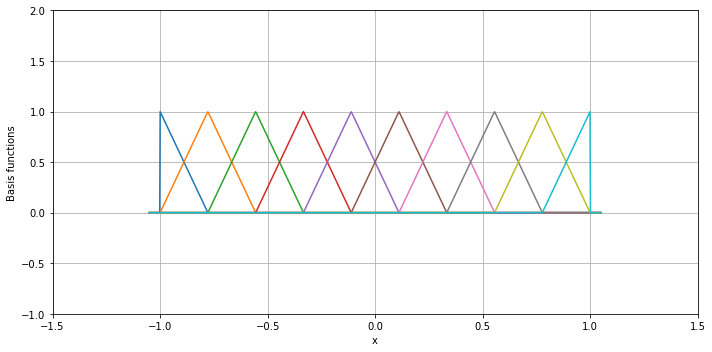
\includegraphics[width = 0.6\textwidth]{img/FEMBasisFunctions.png}
    \caption{The finite element basis functions over the domain $\Omega = [a,\:b]$ for $N=9$.}
    \label{fig:fembases}
\end{figure}

\subsection{Framework And Structure of The VPINNs Scheme}\label{sec:vpinnsframework}

\subsubsection{Multilayer Perceptron}\label{sec:vpinnsmlp}
Let $\mathcal{N}$ be the space of a fully-connected multilayer perceptron (MLP) with 1 node at the input layer, $N$ nodes on each of $D$ hidden layers, and 2 nodes at the output layer as depicted in \autoref{fig:vpinndeepmlp}. The 2 dimensional output represents the real and the imaginary parts of the solution: $u_N(x) = u_{N,\;1}(x) + \imath u_{N,\;2}(x)$. In case of shallow networks, it could be easily shown that this will be the same as using complex model parameters. For this generic structure of the MLP, each element of the the 2-dimensional solution could be expressed as
\begin{equation}
    \label{eq:vpinngeneric}
    u_{N,\;i} = c_0^i + \sum_{j=1}^{N}{c_j^i \sigma(h^{D} \circ h^{D-1} \circ \cdots \circ h^1(x))},
\end{equation}
where $\sigma (x)$ is a non-linear activation function, $h^1_i = \sigma(w^1_i x + b^1_i)$, and
$h^d_i = \sigma(\sum_{n=1}^{N}{w^d_{i, n} h^{d-1}_n} + b^d_i)$ for $d = 2, \cdots, D$.

\begin{figure}[h!]
    \centering
    \begin{subfigure}[b]{0.45\textwidth}
        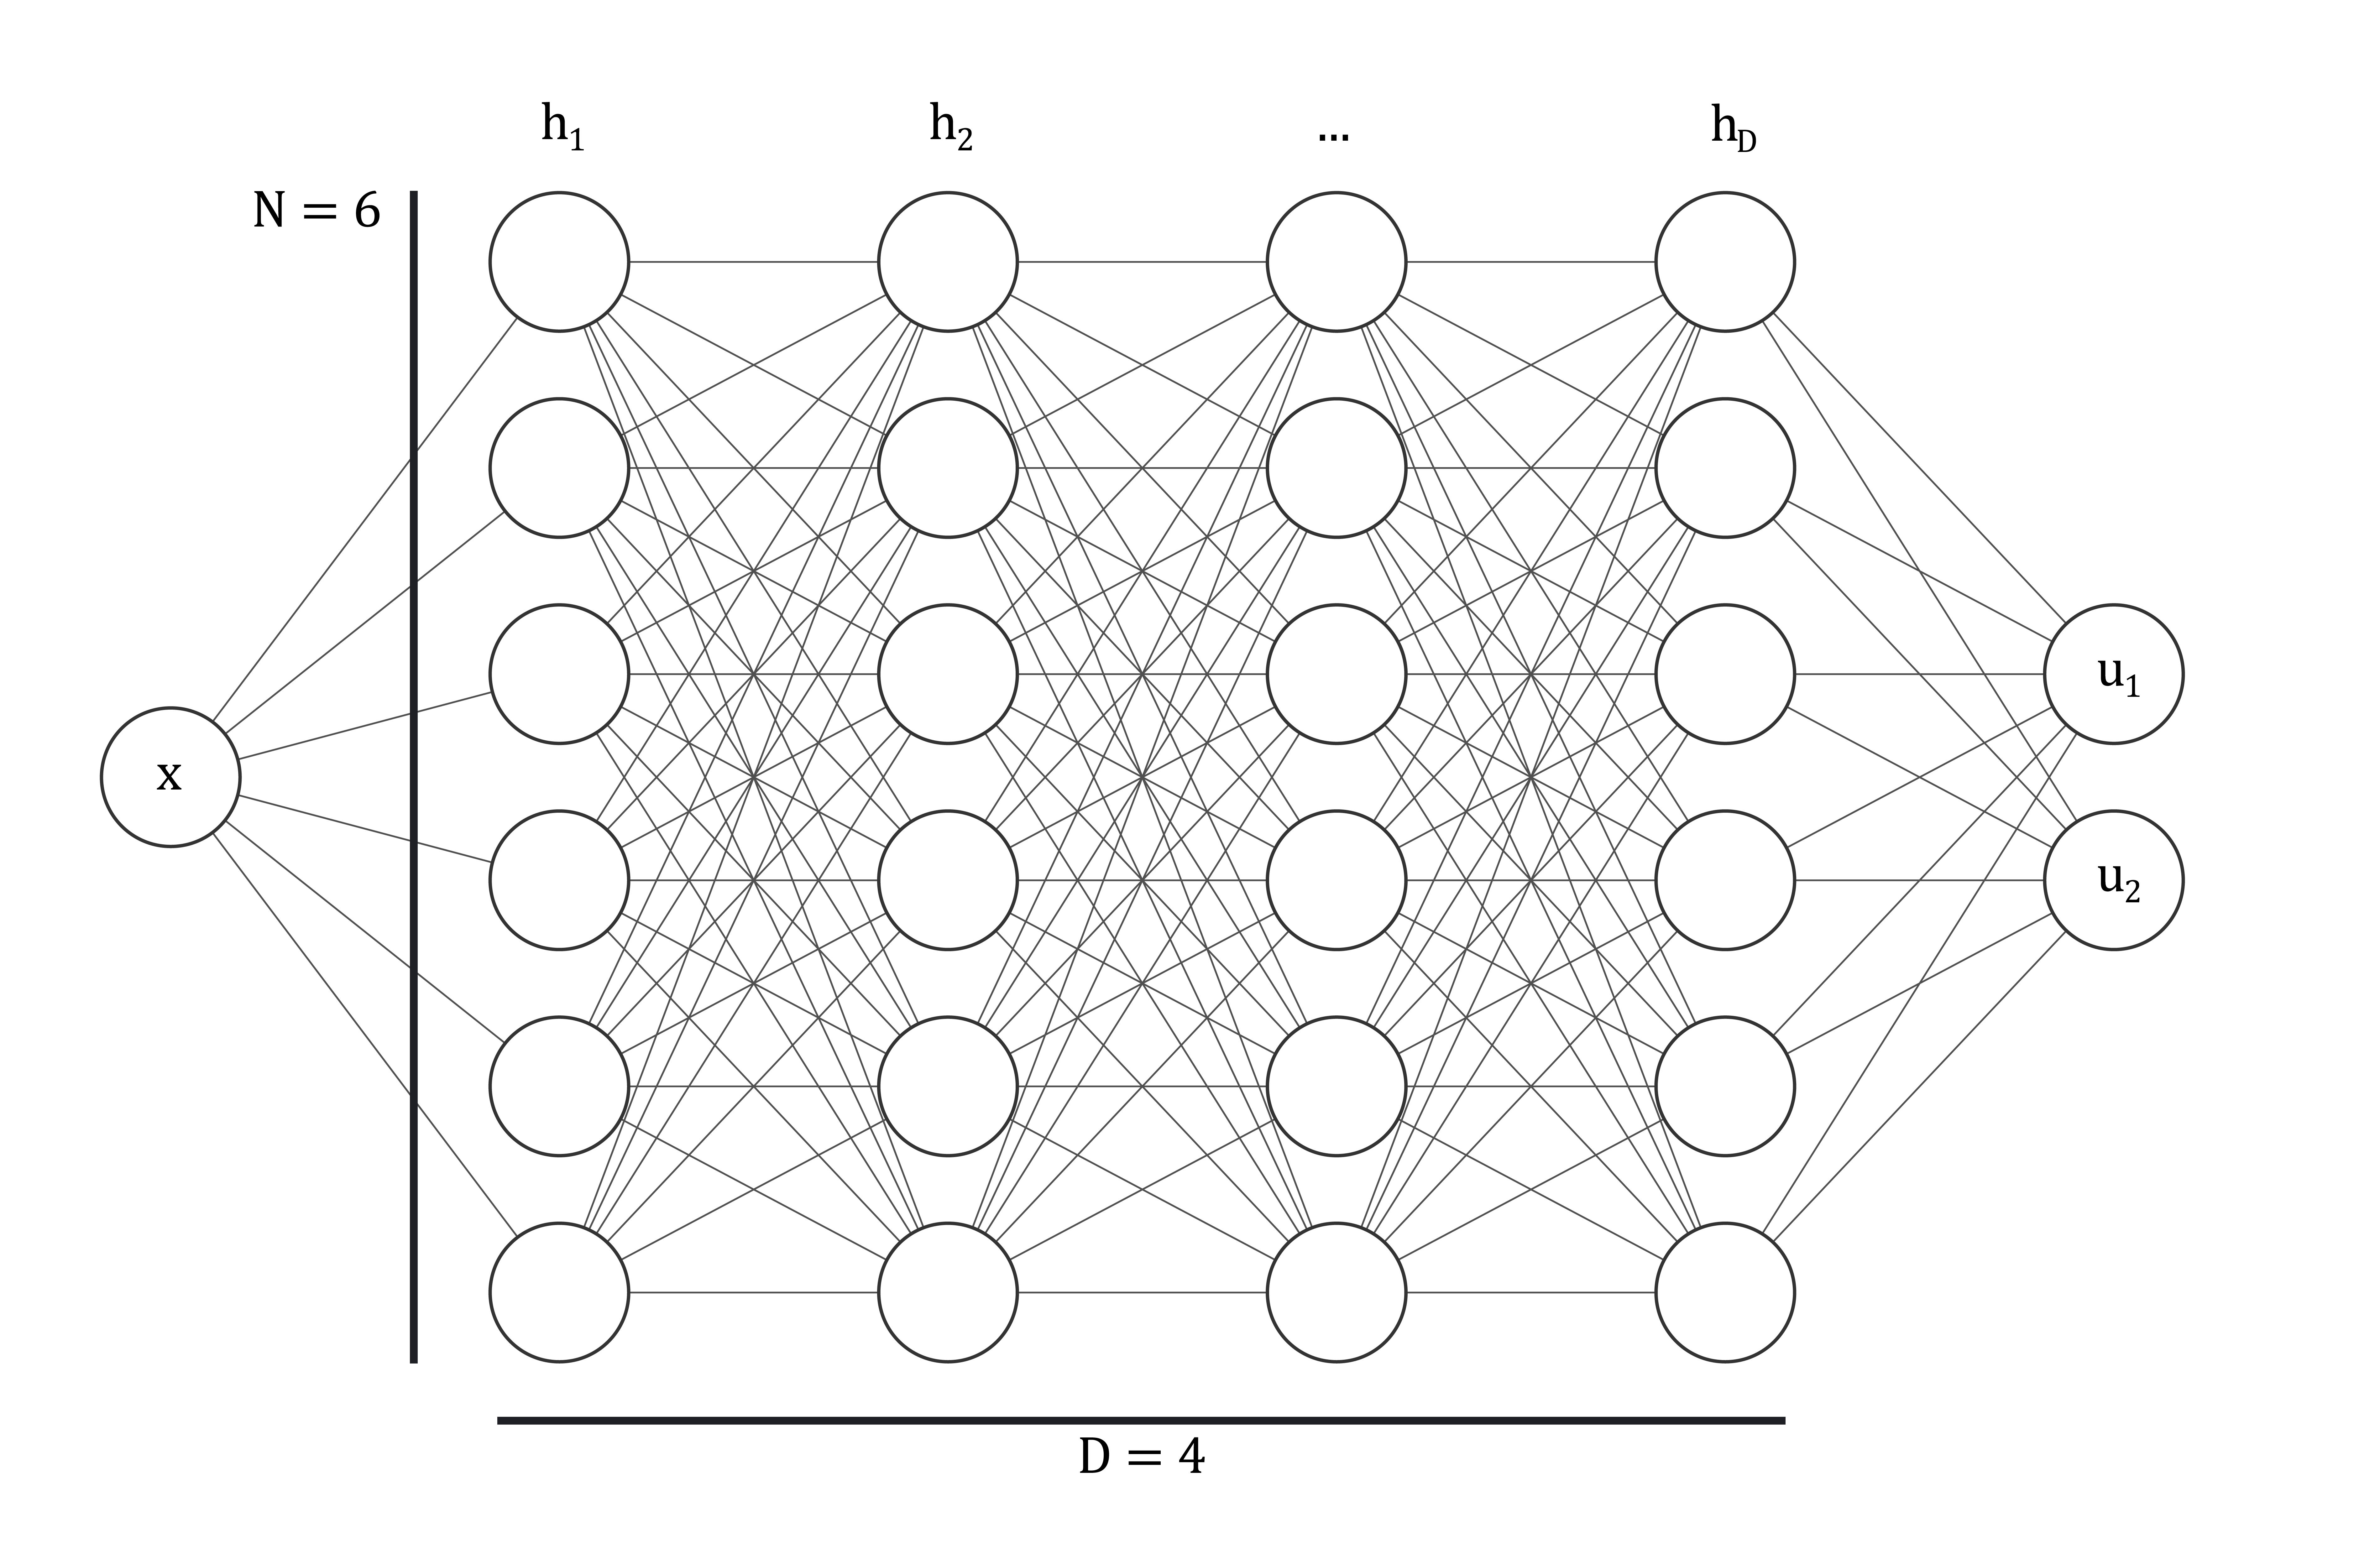
\includegraphics[width=\textwidth]{img/DeepMLP.png}
        \caption{Generic mulilayer perceptron with 4 hidden layer and $N=6$.}
        \label{fig:vpinndeepmlp}
    \end{subfigure}
    \hfill
    \begin{subfigure}[b]{0.45\textwidth}
        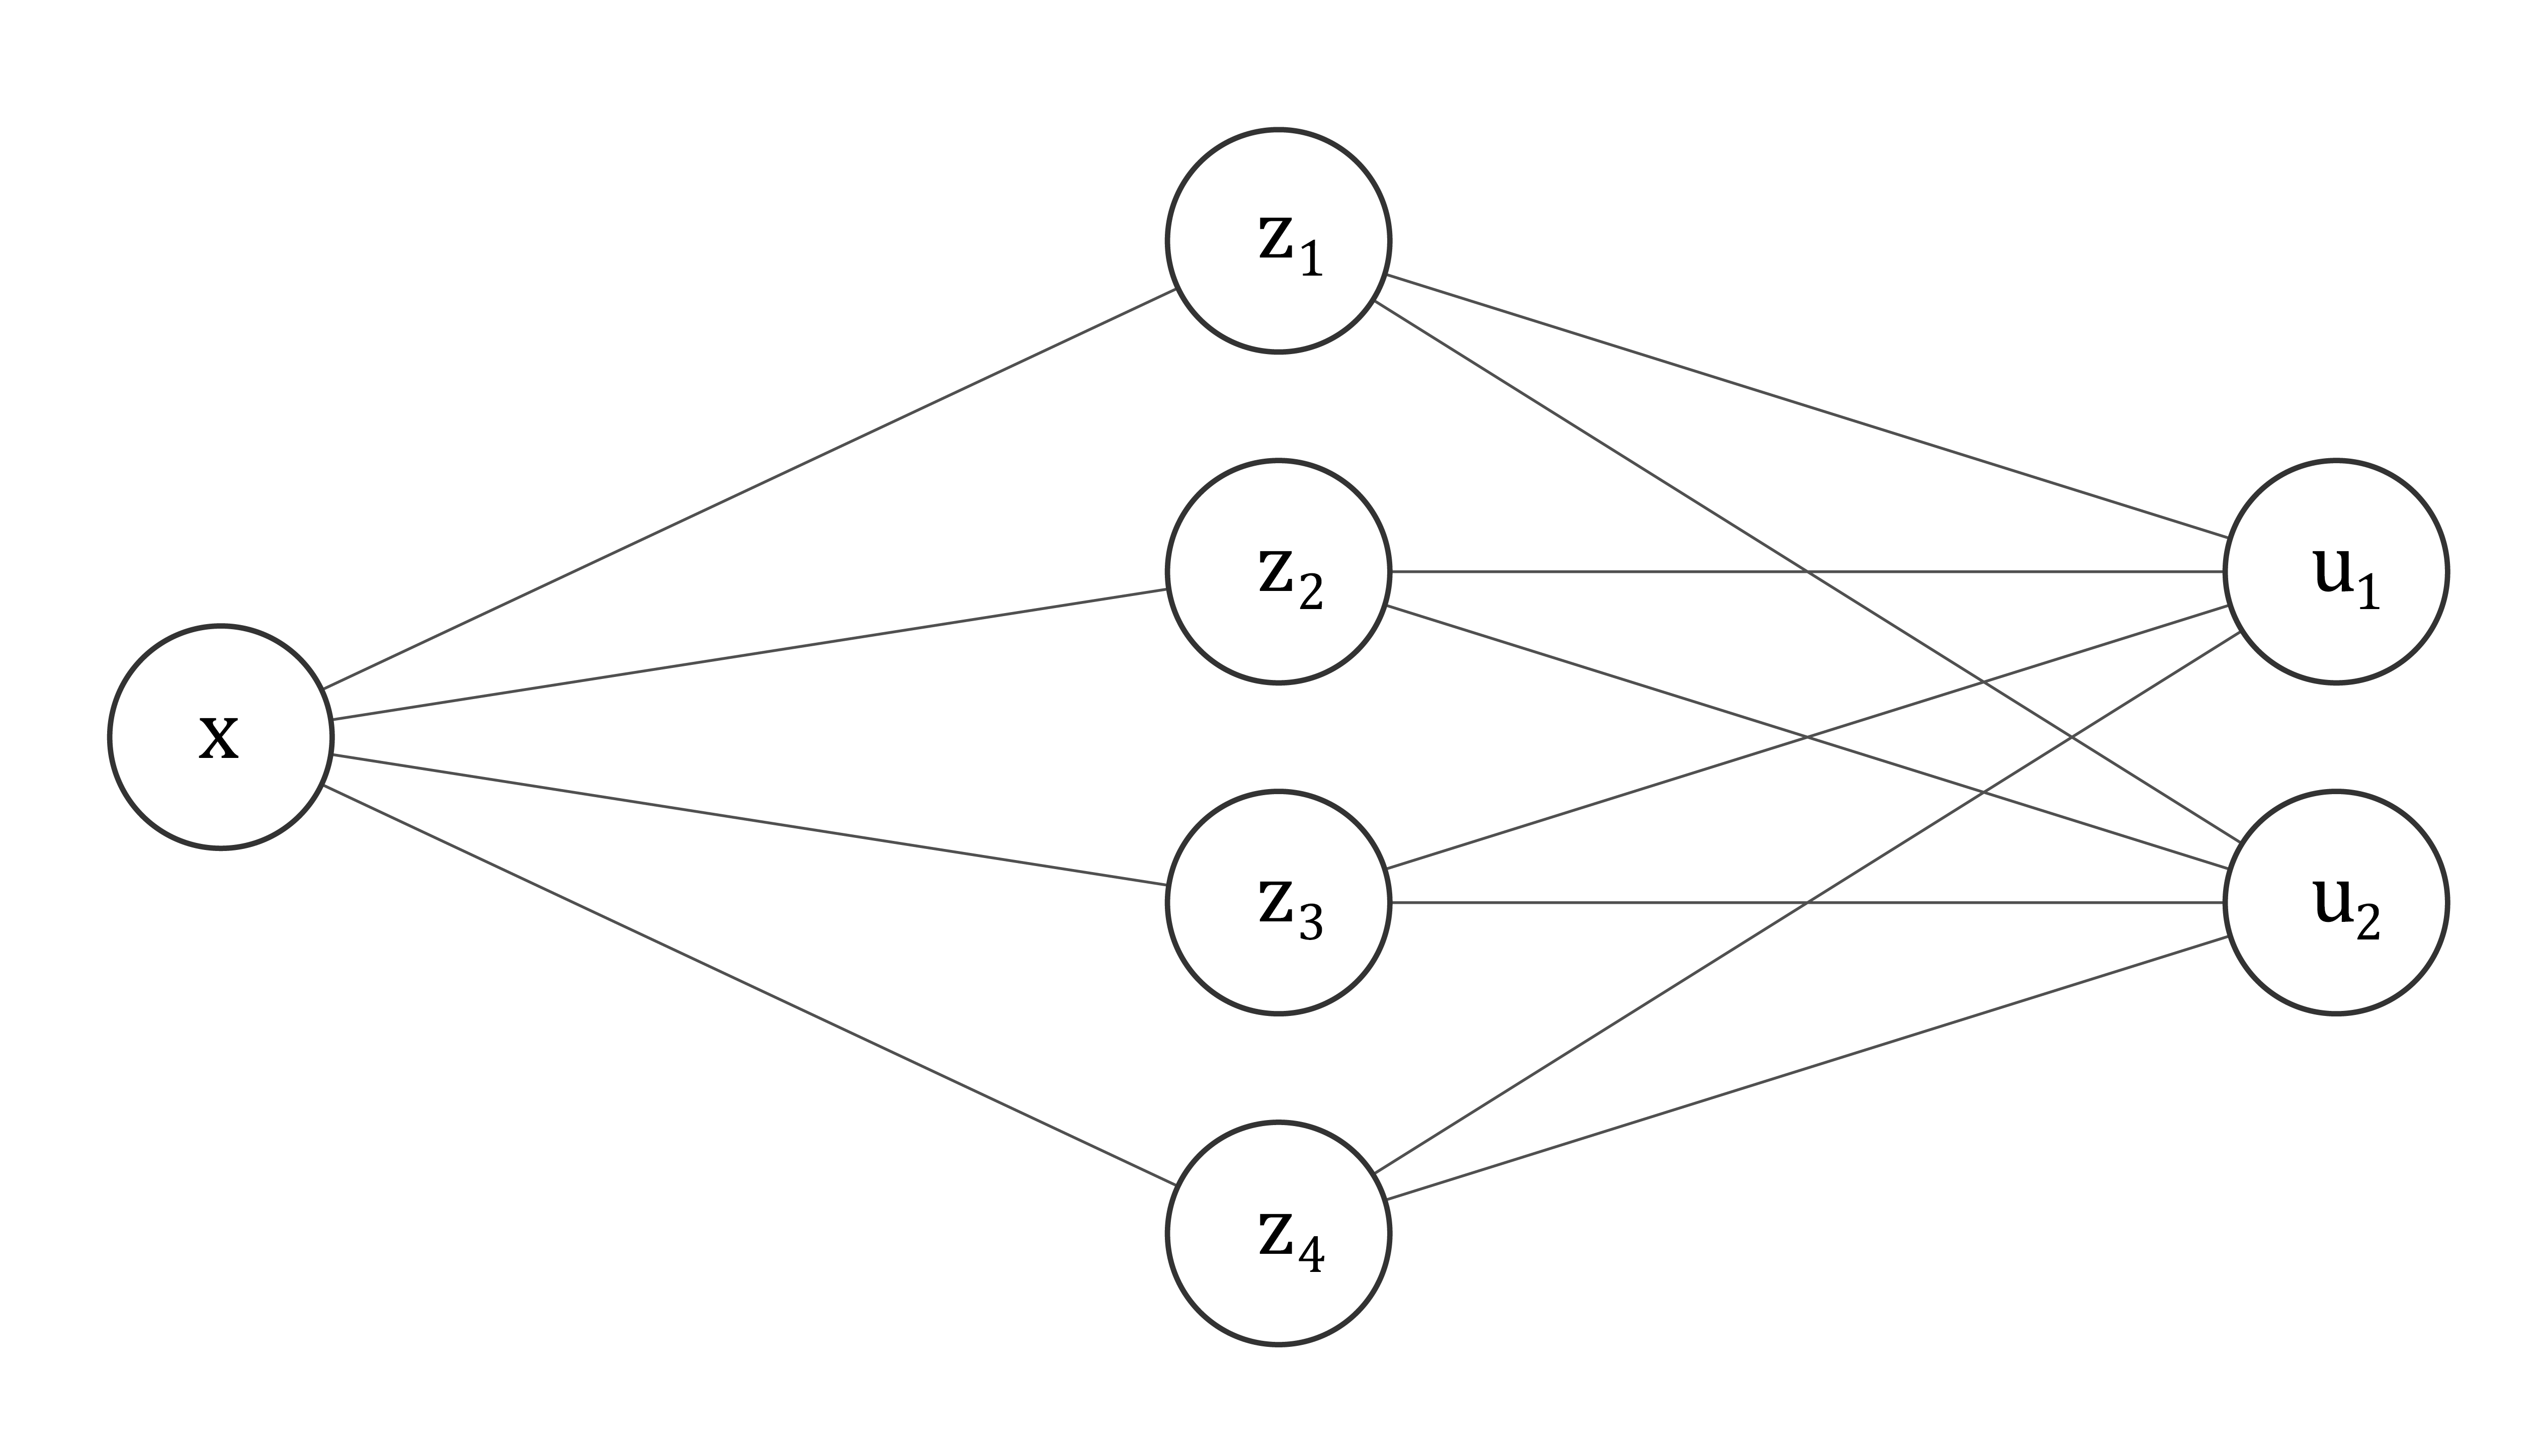
\includegraphics[width=\textwidth]{img/ShallowMLP.png}
        \caption{Shallow multilayer perceptron with $N=3$.}
        \label{fig:vpinnshallowmlp}
    \end{subfigure}
\end{figure}

With this structure, the network has $2N$ parameters for the first hidden layer, $(D-1)(N^2+N)$ parameters for other hidden layers, and $2N+2$ parameters for the last year, which sums up as
\begin{equation}
    \label{eq:vpinnsparameters}
    N_p = (D-1)N^2+(D+3)N+2,
\end{equation}
where $N_p$ is total number of parameters of the network.

\subsubsection{Variational Formulation for VPINNs}\label{sec:vpinnsformulation}
Let $V_K = span(v_1, v_2, \cdots, v_K)$ be the space of the test functions. The helmholtz impedance problem in the context of VPINNs is defined as finding $u_{\mathcal{N}} \in \mathcal{N}$ such that the loss function
\begin{equation}
    \label{eq:lossfunction}
    \mathcal{L}^{(2)}(u_{\mathcal{N}}) = \frac{1}{K} \sum_{k=1}^{K}{|R_k^{(2)} - F_k|^2}
\end{equation}
is minimized, where
\begin{equation}
    \label{eq:vpinnlhs}
    R_k^{(2)} = \int_{a}^{b}{u'_{\mathcal{N}}v'_k} - k^2 \int_{a}^{b}{u_{\mathcal{N}}v_k} - (g_a + \imath ku_{\mathcal{N}}(a))v_k(a) - (g_b + \imath ku_{\mathcal{N}}(b))v_k(b),
\end{equation}
\begin{equation}
    \label{eq:vpinnrhs}
    F_k = \int_{a}^{b}{fv_k}.
\end{equation}

\subsubsection{Least Squares Initialization}\label{sec:lsinit}
An important factor for training a neural network is the initialization of the parameters. Because of the unsupervised nature of VPINNs, the initialization could be more important and more helpful than for the networks with supervised learning purposes. Some methods such as new reptile initialization based physicis-informed neural network (NRVPINN)~\cite{liu2021init} have been proved to be substantially helpful to the training. In this work, we investigate the effect of a specialized least-squares based initialization for the case of shallow networks which is described in this section. Considering N nodes in the hidden layer, we initialize the weight of this layer as $w^{1}_{i} = k$, where $k$ is the wave number of the equation. The bias of this layer initialized as $b^{1}_{i} = -w^{1}_{i} x^{*}_{i}$, where $x^{*}_{i}$ for $i=1,2,...,N$ is uniformly distributed on the interval $\Omega$. With this initialization, the output of the shallow network could be expressed As
\begin{equation}
    u_{N,\;i} = c_0^i + \sum_{j=1}^{N}{c_j^i h^1_j} = c_0^i + \sum_{j=1}^{N}{c_j^i \sigma(k(x-x^{*}_j))}.
\end{equation}
Initializing the biases of the last layers with zeros, i.e $c_0^i = 0$, the weights of the last layer are initialized as the real and imaginary part of the least-square solution of the system of equations $A\underline{c}=\underline{f}$, where $A$ is a complex $K \times N$ matrix with $A_{i, j}=a(\phi_i, h^1_j)$ and $f_i = b(\phi_i)$ for $i=1,2,...,K$. An example of such an initialization is given in \autoref{fig:lsinit} for $N=K=20$ and the wave number $k=16$. We can see that by such an initialization we can take advantage of the information we have about the frequency of oscillations of the solution to get a very good frist guess. However, one needs to put more thought into it for implementing this initialization for deep networks, or other types of source functions. Furthermore, the method could be improved by choosing $x^{*}$'s adaptive to the wave number $k$, since these are the x-intercepts of the bases of the initial solution.

\begin{figure}[h!]
    \centering
    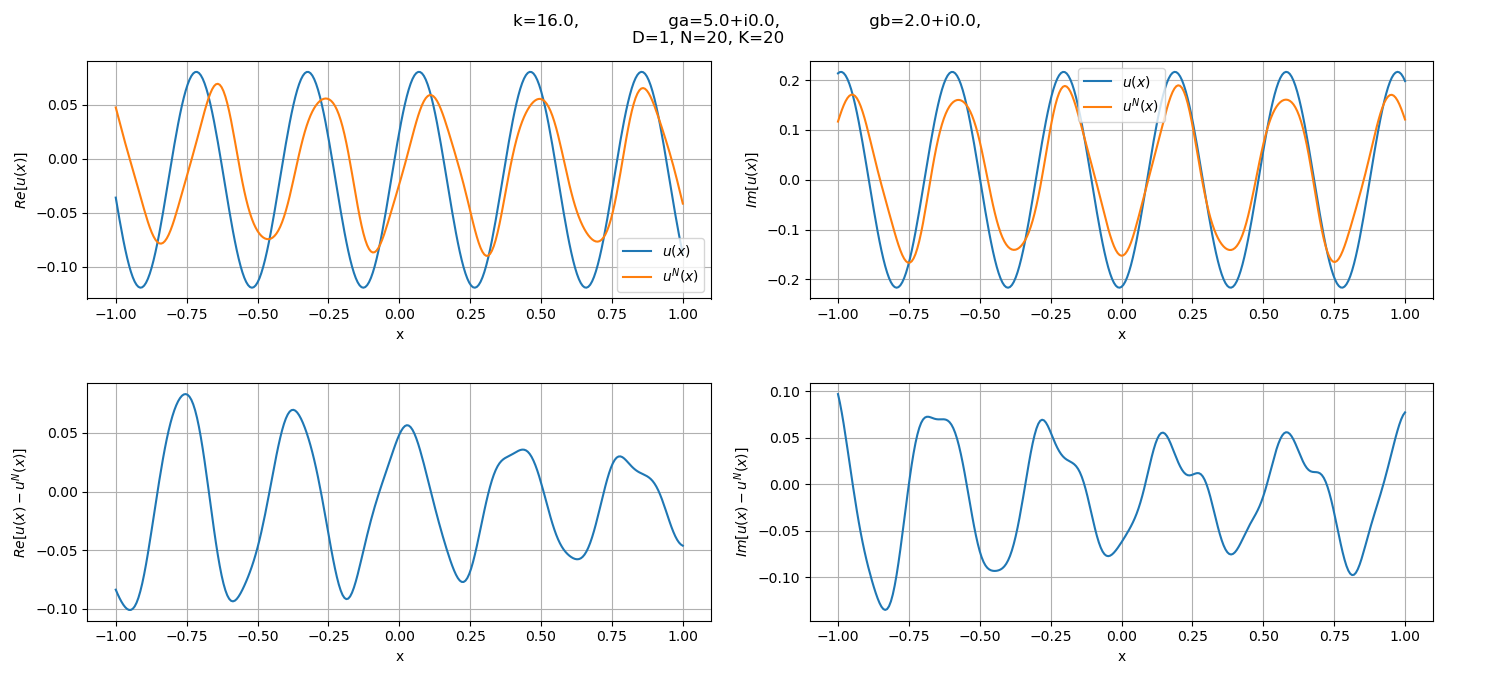
\includegraphics[width=.7\textwidth]{img/VPINN-lsinit.png}
    \caption{Example of the least-squares initialization for a shallow neural network.}
    \label{fig:lsinit}
\end{figure}

\subsubsection{Quadrature Rules for Integrations}\label{sec:quadraturerules}
The integrals in Equations \ref{eq:vpinnlhs} and \ref{eq:vpinnrhs} are evaluated using the Legendre-Gauss-Lobato quadrature rule, which for an arbitrary 1D function $f(x)$ is defined as
\begin{equation}
    \label{eq:quadrature}
    \int_a^bf(x)dx = \sum_{i=1}^N{w_if(x_i)},
\end{equation}
where $w_1$ to $w_N$ are quadrature weights, and $x_1$ to $x_N$ are quadrature points in the interval $\Omega = [-1, +1]$, including the endpoints. When using test functions with local support (such as finite element hat functions defined in \autoref{eq:fembasisfuncs}), the quadrature points should be chosen carefully. Since these test functions are only defined in a subset of the whole domain, choosing global quadrature points results in a poor approximation of the integral. Therefore, we use local quadrature points to evaluate the integrals that invovle test functions with local support, and global quadrature points, when the function being integrated is globally defined.

\section{Results And Discussion}\label{sec:results}
The frameworks described in the previous section are implemented and their results are presented and discussed in this section. We define the error of the solution as the $H^1{(\Omega)}$ norm of difference between the analytical solution $u(x)$, and the solution of the numerical scheme $u_N(x)$:
\begin{equation}
    \label{eq:H1error}
    ||u(x) - u_N(x)||_{H^1{(\Omega)}} = ||u(x) - u_N(x)||_{L^2{(\Omega)}} + ||u'(x) - u'_N(x)||_{L^2{(\Omega)}},
\end{equation}
where
\begin{equation}
    \label{eq:L2error}
    ||f(x)||_{L^2{(\Omega)}} = \begin{pmatrix} \int_{\Omega}{|f(x)|^2dx} \end{pmatrix}^{1/2},
\end{equation}
and use this error as a measure to evaluate the solution from each numerical scheme.

\begin{figure}[h!]
    \centering
    \begin{subfigure}[b]{0.7\textwidth}
        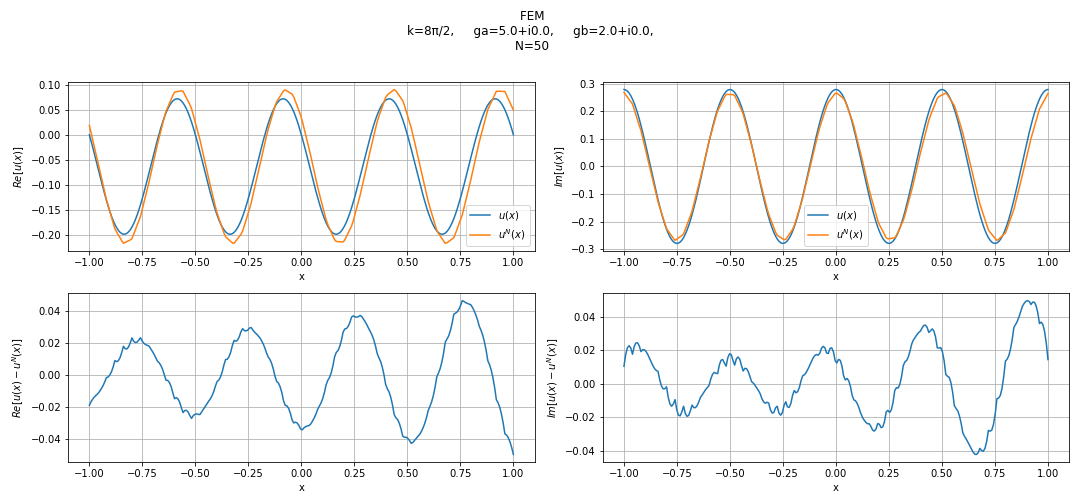
\includegraphics[width=\textwidth]{img/FEM-Const-MidFreq-N0050-sol.png}
        \caption{$u_N(x)$.}
    \end{subfigure}
    \vfill
    \begin{subfigure}[b]{0.7\textwidth}
        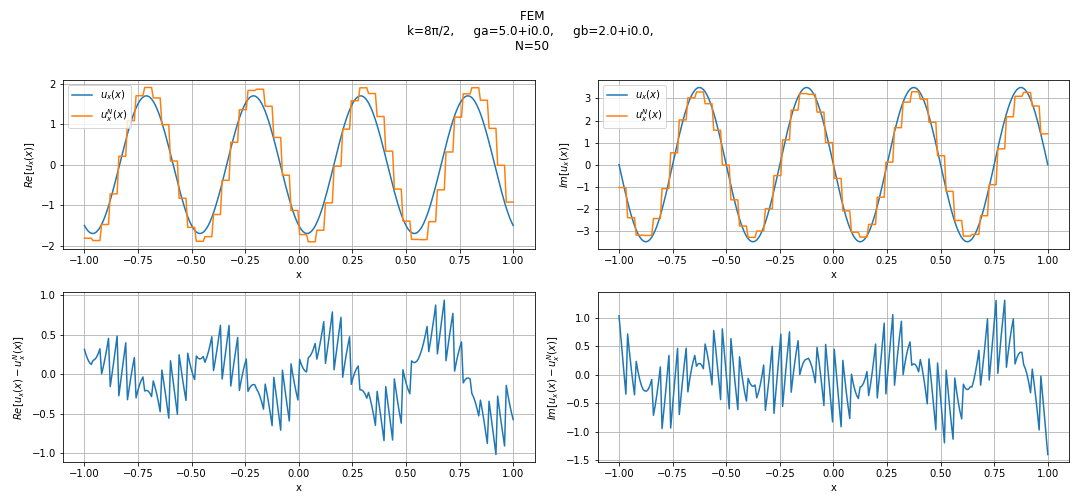
\includegraphics[width=\textwidth]{img/FEM-Const-MidFreq-N0050-der.png}
        \caption{$u'_N(x)$.}
    \end{subfigure}
    \caption{$u_N(x)$ and $u'_N(x)$ plotted against the exact solution for a relatively moderate $k$ and $N=50$. On each subfigure, the bottom row represents the difference between the numerical and exact solutions. The source function has a constant value of $f(x)=10$, and the other parameters are indicated on the plots.}
    \label{fig:femMidfreqN050}
\end{figure}

\subsection{Finite Element Scheme}\label{sec:femresults}
Implementing the framework described in \autoref{sec:femframework}, we investigated the results of the finite element scheme for the Helmholtz impedance problem with different wave numbers. The results for a relatively moderate $k$ validated against the exact solution are presented in Figures \ref{fig:femMidfreqN050} and \ref{fig:femMidfreqN100}. These plots show how using a finer mesh (bigger $N$) on the domain improves the quality of the solution. The same trend has been observed for other $k$'s.

\begin{figure}[h!]
    \centering
    \begin{subfigure}[b]{0.7\textwidth}
        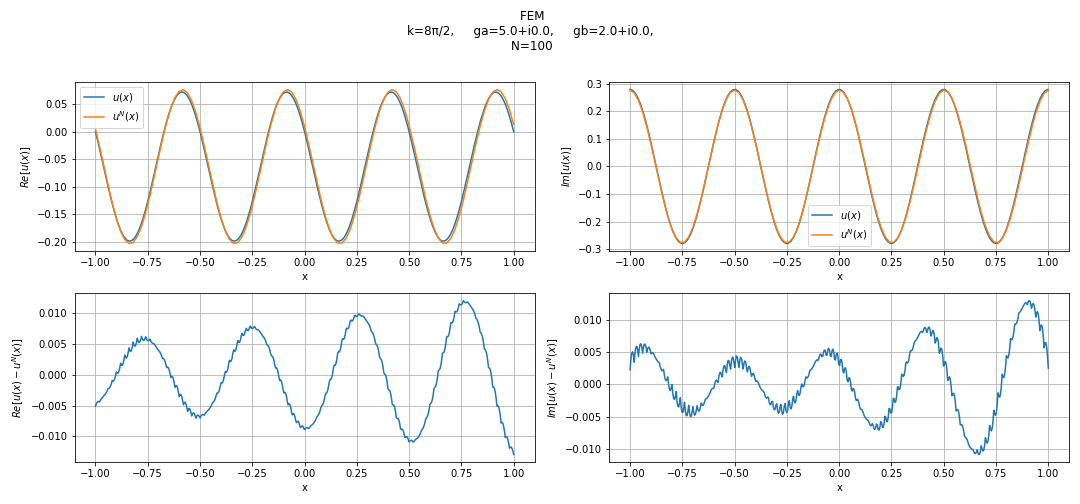
\includegraphics[width=\textwidth]{img/FEM-Const-MidFreq-N0100-sol.png}
        \caption{$u_N(x)$}
    \end{subfigure}
    \vfill
    \begin{subfigure}[b]{0.7\textwidth}
        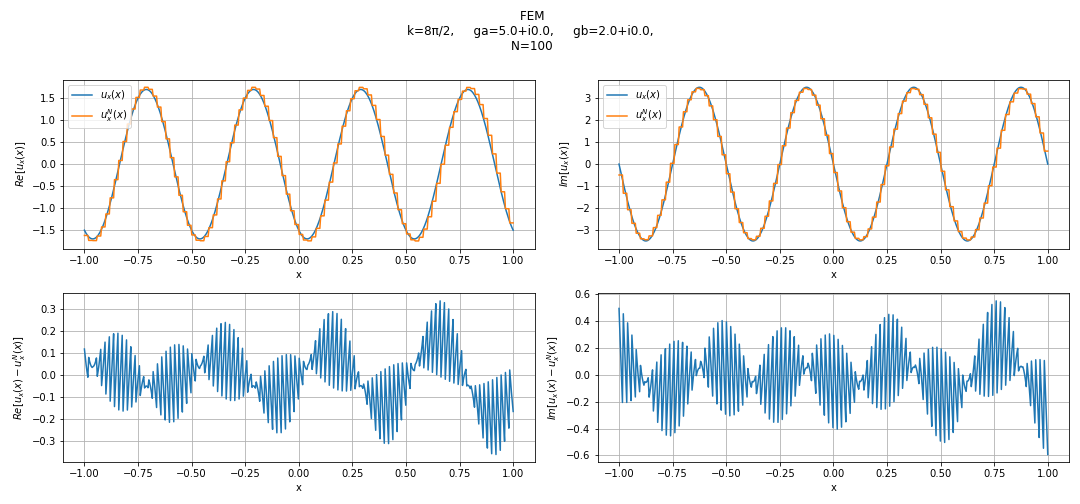
\includegraphics[width=\textwidth]{img/FEM-Const-MidFreq-N0100-der.png}
        \caption{$u'_N(x)$}
    \end{subfigure}
    \caption{$u_N(x)$ (a) and $u'_N(x)$ (b) plotted against the exact solution for a relatively moderate $k$ and $N=100$. On each subfigure, the bottom row represents the difference between the numerical and exact solutions. The source function has a constant value of $f(x)=10$, and other parameters are indicated on the figures.}
    \label{fig:femMidfreqN100}
\end{figure}

However, for larger values of $k$, there is an issue with this method. From the nature of the equation we know that for larger $k$'s, we have more oscillations in the solution. Since the finite element scheme estimaes the solution with piecewise linear basis functions in a uniform mesh, the resulting numerical solution will be piecewise linear. This will require a minimum number of grid points on each oscillation for the estimation to have a decent accuracy. Consider the solution in \autoref{fig:femMidfreqN100} where we used 100 grid points. If we wanted to estimate this function with 8 grid points, for instance, it was not possible to even capture the general shape of the function. This phenomenon is the major observation in \autoref{fig:femorder}, where the H1-error of the numerical solution is plotted against mesh refinement parameter, $N$, for different values of $k$. For each constant $k$, there is no improvement in the error as we refine the mesh until a certain $N$, which we call $N_c$. However, for $N > N_c$, we can see the first-order accuracy of the method as expected. Another important observation is that the value of $N_c$ increases with increasing $k$, which means that for high values of $k$, the improvement in the accuracy only exists for extremely fine meshes.

\begin{figure}[h!]
    \centering
    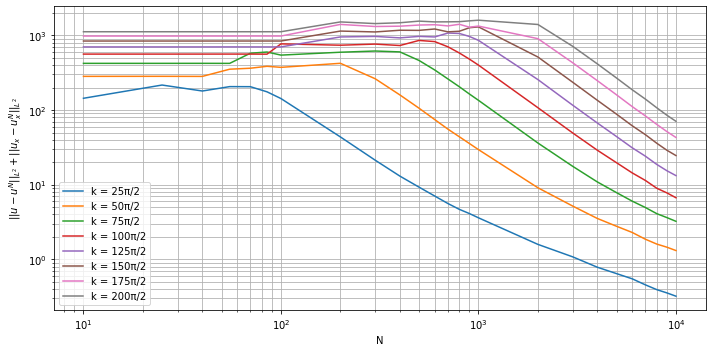
\includegraphics[width=.7\textwidth]{img/FEM-Order-Homog-H1.png}
    \caption{Order of accuracy of the FEM scheme for different values of $k$.}
    \label{fig:femorder}
\end{figure}

\subsection{VPINNs Scheme}\label{sec:vpinnsresults}
Implementing the framework explained in \autoref{sec:vpinnsframework}, we investigated the performace of this scheme for different network structures, different activation functions, different initialization techniques, different formulations, and for different wave numbers $k$. The Adam optimizer~\cite{adamoptimizer} is used for all the trainings. Except for the results presented in \autoref{sec:lsinitresults}, the weights of each layer are initialized using the normal Xavier initialization~\cite{xavierinitialization}, and the biases are initialized using a uniform distribution in the domain $\Omega$. This initialization, when compared to the least-squares initialization presented in \autoref{sec:lsinit}, will be called random initialization. In all the trainings except the ones with the coercive variational formulation presented in \autoref{sec:coerciveformulation} where the first $K$ Legendre polynomials are used, we use the local hat functions defined by \autoref{eq:fembasisfuncs} for the test functions. Each training is done multiple times to ensure independance from randomness and the best one is selected for comparisons. The biggest learning rate $lr$ that ensures convergence and accuracy for most of the networks being compared turned out to be $5e{-02}$ (unless stated otherwise), which is kept fix in all the comparisons.

\subsubsection{Shallow Networks} \label{sec:vpinnsshallowresults}

\begin{figure}[h!]
    \centering
    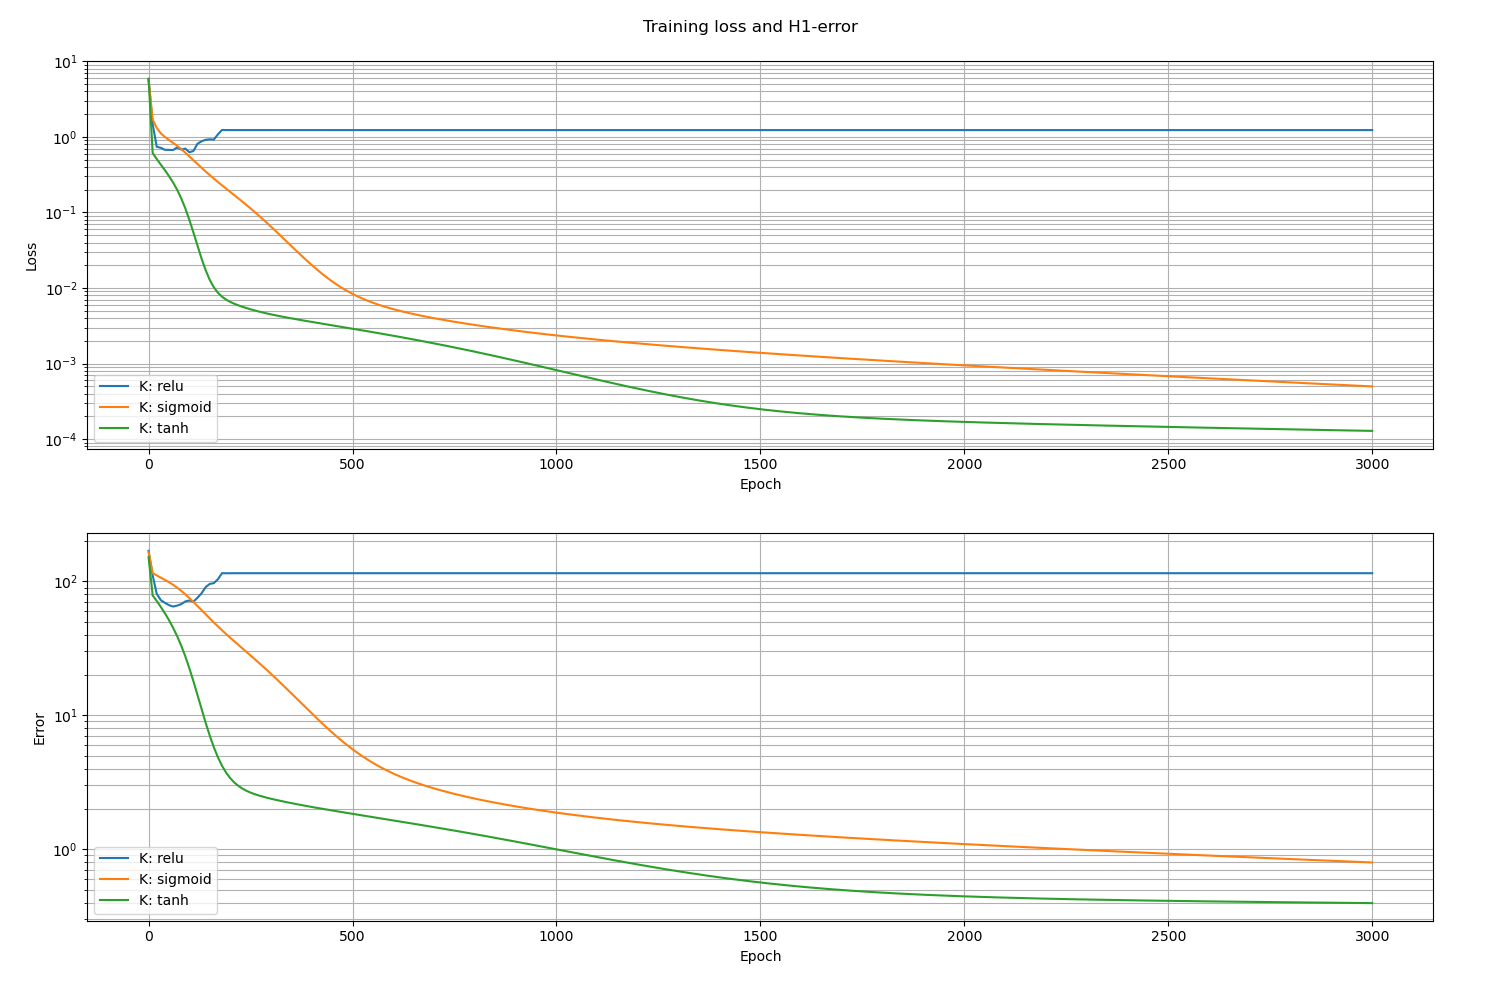
\includegraphics[width=.7\textwidth]{img/VPINN-Comparison-Activation.png}
    \caption{Training loss and H1-error of a shallow network with $N=10$ and $K=10$ with different activation functions for $k=1.0$.}
    \label{fig:activationfunctions}
\end{figure}

We start with shallow neural networks with only one hidden layer, i.e. $D=1$. We use the local hat functions presented in \autoref{eq:fembasisfuncs} as test functions, and train a network with $N=10$ and 10 test functions ($K=10$) with different types of activation functions for a low wave number. The loss functions and the errors are compared in \autoref{fig:activationfunctions}. The learning rate is $1e{-01}$ for all the activation functions. We can see that the hyperbolic tangent activation function outperforms the sigmoid activation function for our setup both in terms of accuracy and the convergence rate. Regarding the ReLU activation function, there are some issues inherited with this set-up of networks. If we train the weights and biases of the hidden layer, these parameters drive the threshold of each ReLU outside of the support domain of the test functions, and the gradient of the loss with respect to these parameters goes to zero, so technically, the hidden neurons will be lost one by one. As done in \cite{liu2021}, it could be easily shown that in case of the ReLU activation function, the weights of the hidden layer are redundent for this kind of networks and it is suggested to set the weights to 1. To address the issue with ReLU activation function, the network is trained with fixed biases being uniformly distributed in the domain $[a, b]$ and weights fixed to 1, and the training could be completed without this issue. However, by fixing the parameters of the hidden layer and the ReLU activation function, this framework has no advantage over the original FEM scheme in case of capability and adaptability. In the rest of the experiments, the hyperbolic tangent activation function is used for the trainings.

\begin{figure}[h!]
    \centering
    \begin{subfigure}[b]{0.48\textwidth}
        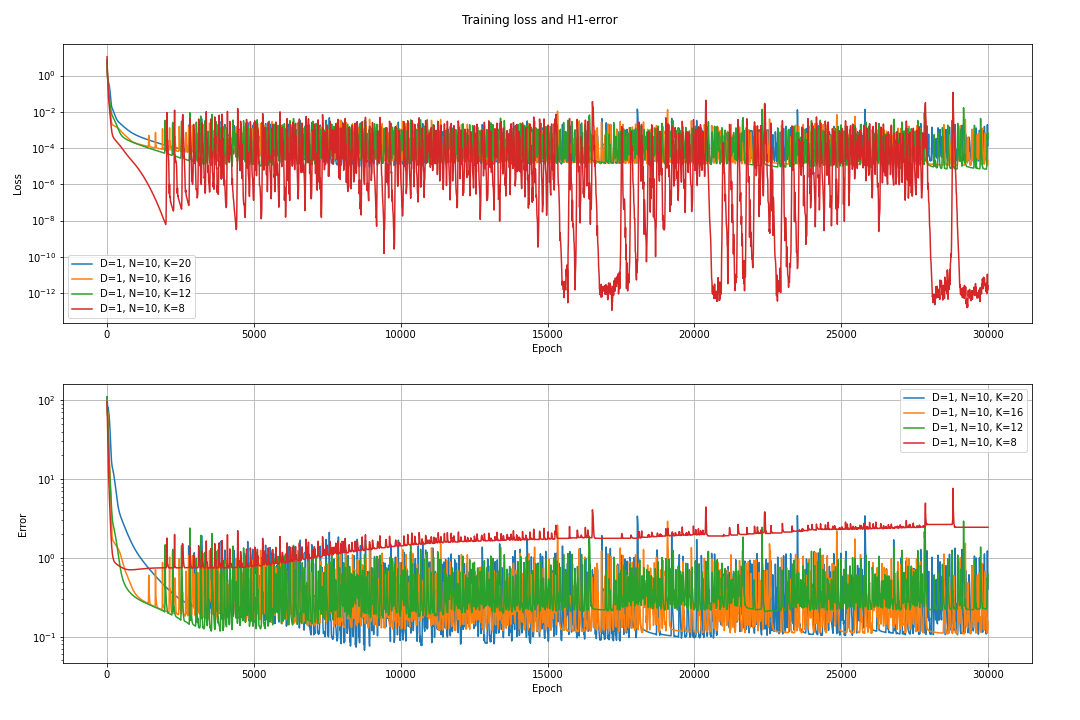
\includegraphics[width=\textwidth]{img/VPINN-Comparison-k2increaseK.png}
        \caption{$k=2$.}
        \label{fig:vpinnsk2increaseK}
    \end{subfigure}
    \hfill
    \begin{subfigure}[b]{0.48\textwidth}
        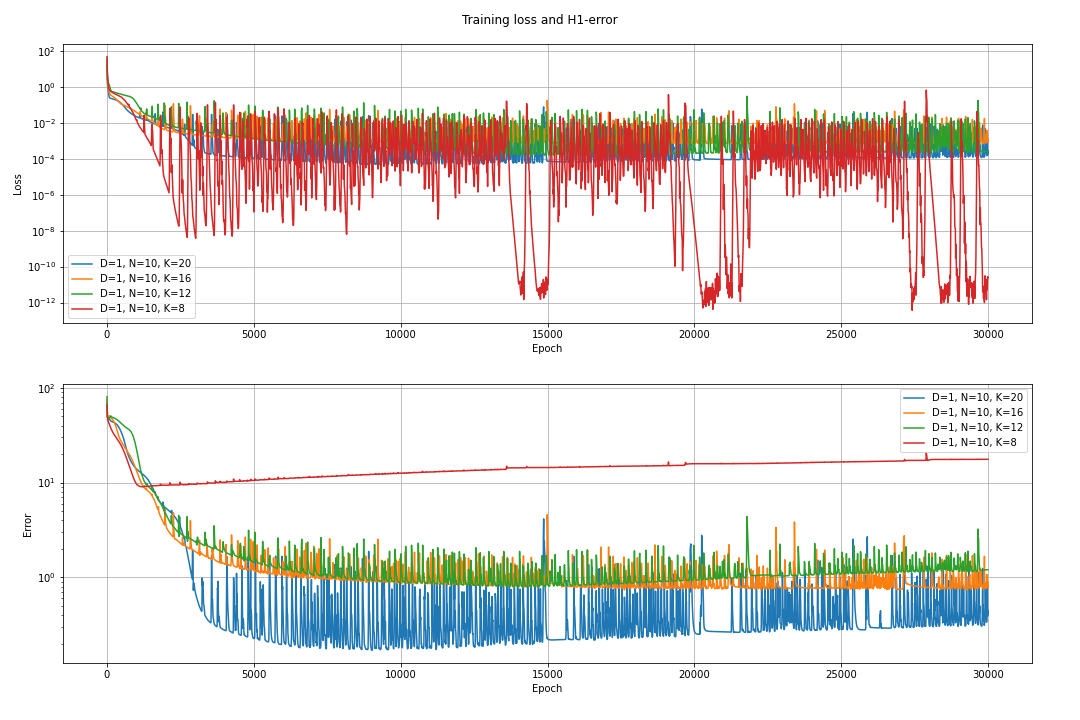
\includegraphics[width=\textwidth]{img/VPINN-Comparison-k4increaseK.png}
        \caption{$k=4$.}
        \label{fig:vpinnsk4increaseK}
    \end{subfigure}
    \vfill
    \begin{subfigure}[b]{0.48\textwidth}
        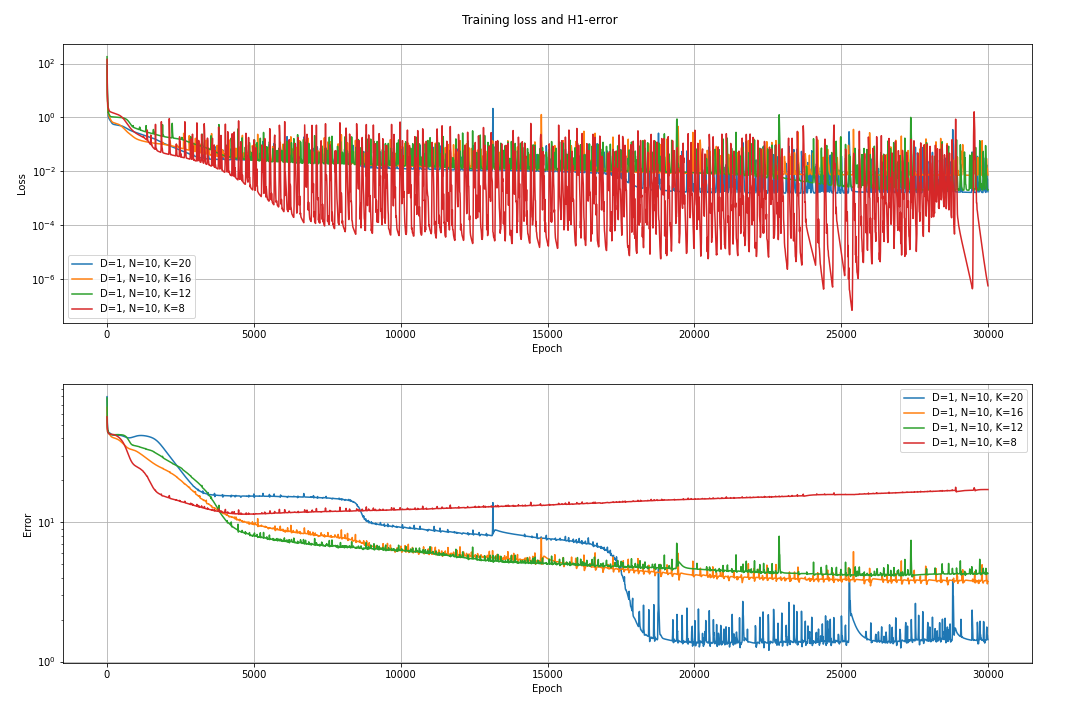
\includegraphics[width=\textwidth]{img/VPINN-Comparison-k6increaseK.png}
        \caption{$k=6$.}
        \label{fig:vpinnsk6increaseK}
    \end{subfigure}
    \hfill
    \begin{subfigure}[b]{0.48\textwidth}
        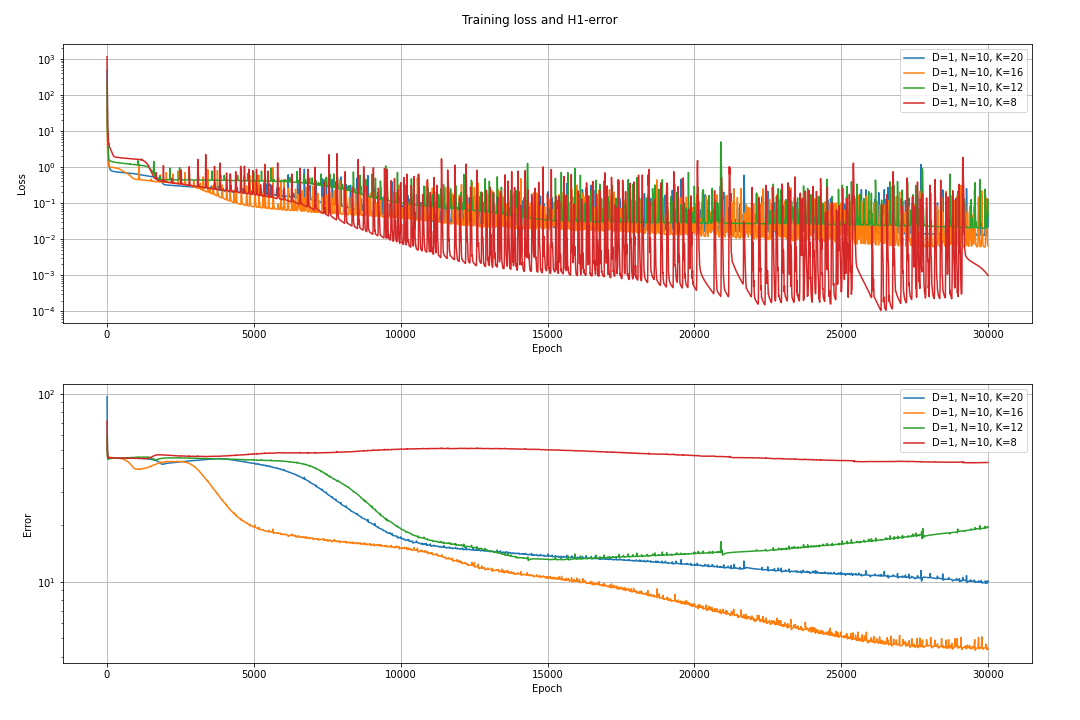
\includegraphics[width=\textwidth]{img/VPINN-Comparison-k8increaseK.png}
        \caption{$k=8$.}
        \label{fig:vpinnsk8increaseK}
    \end{subfigure}
    \caption{Training loss and H1-error with fixed network structure and increasing number of test functions for different wave numbers.}
    \label{fig:vpinnsincreaseK}
\end{figure}

In an effort to investigate the effect of increasing the number of test functions on the accuracy and the training of the network, with a fixed width $N=10$, the training is done for different values of $K$. The results are presented in \autoref{fig:vpinnsincreaseK}. For the lowest wave number $k=2$ in \autoref{fig:vpinnsk2increaseK}, we can see that with 8 test functions, the training loss becomes unstable and the H1-error takes an increasing trend after around 2000 epochs. With 12 test functions, this behavior is not observed and the H1-error converges. Increasing the number of test functions to 16, we can see a slight improvement, which does not repeat itself with further increasing the number of test functions to 20. For a higher wave number $k=4$ in \autoref{fig:vpinnsk4increaseK}, we can see the same behavior for 8 test functions but with the difference that the final H1-error keeps being improved with increasing the number of test functions to 20. For the highest wave number $k=8$, we can observe the unstable behavior extends to 12 test functions, and the improvement with increasing the number of test functions becomes more evident. We can conclude that as the wave number increases, more number of test functions will be needed for training the network.

\begin{figure}[h!]
    \centering
    \begin{subfigure}[b]{0.48\textwidth}
        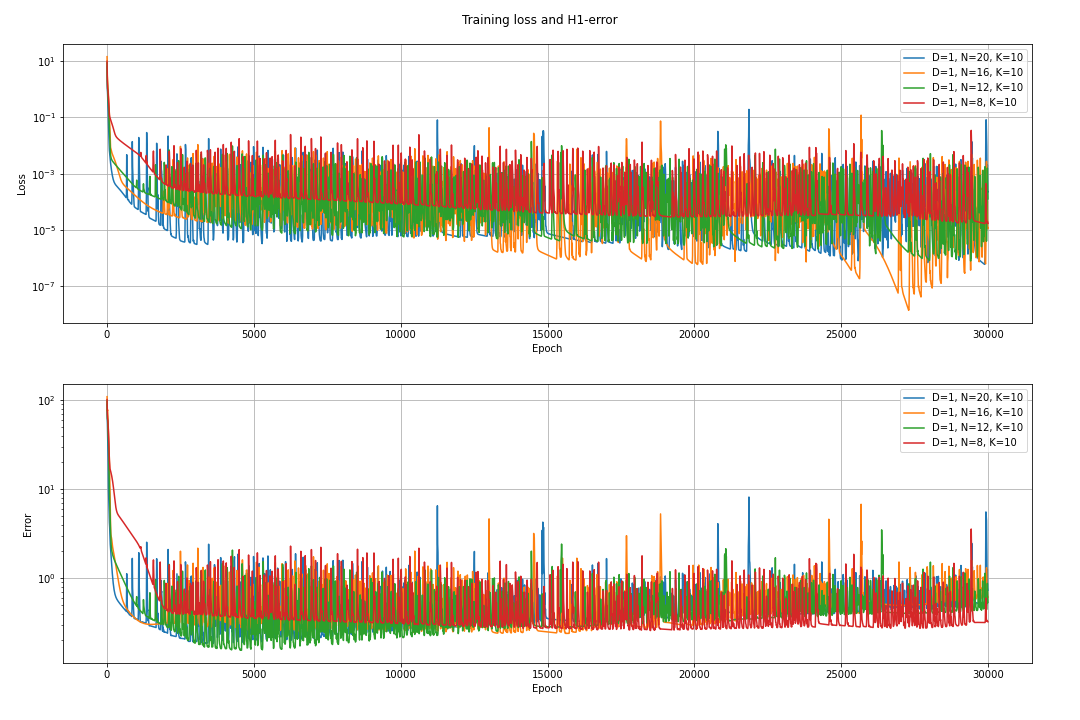
\includegraphics[width=\textwidth]{img/VPINN-Comparison-k2increaseN.png}
        \caption{$k=2$.}
        \label{fig:vpinnsk2increaseN}
    \end{subfigure}
    \hfill
    \begin{subfigure}[b]{0.48\textwidth}
        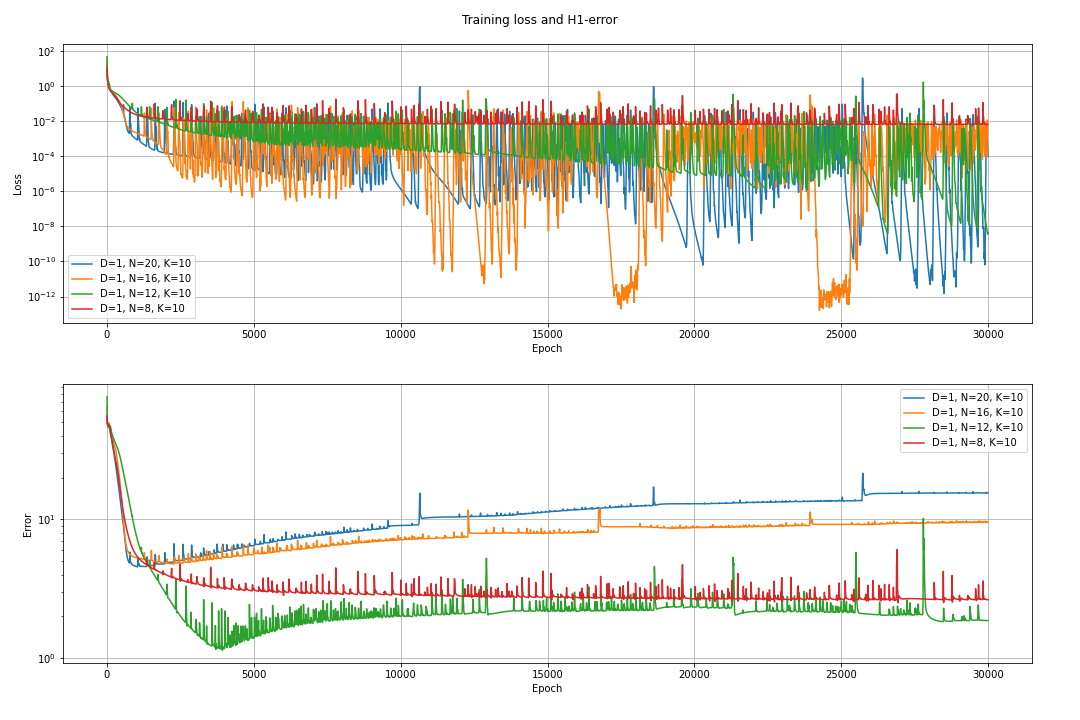
\includegraphics[width=\textwidth]{img/VPINN-Comparison-k4increaseN.png}
        \caption{$k=4$.}
        \label{fig:vpinnsk4increaseN}
    \end{subfigure}
    \vfill
    \begin{subfigure}[b]{0.48\textwidth}
        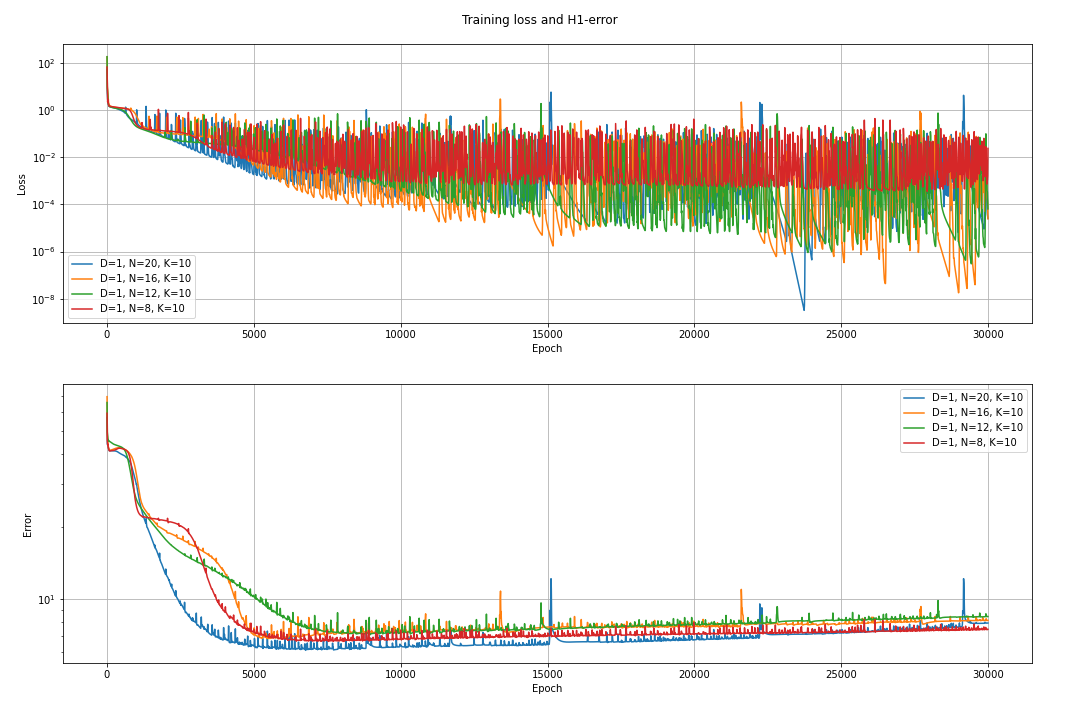
\includegraphics[width=\textwidth]{img/VPINN-Comparison-k6increaseN.png}
        \caption{$k=6$.}
        \label{fig:vpinnsk6increaseN}
    \end{subfigure}
    \hfill
    \begin{subfigure}[b]{0.48\textwidth}
        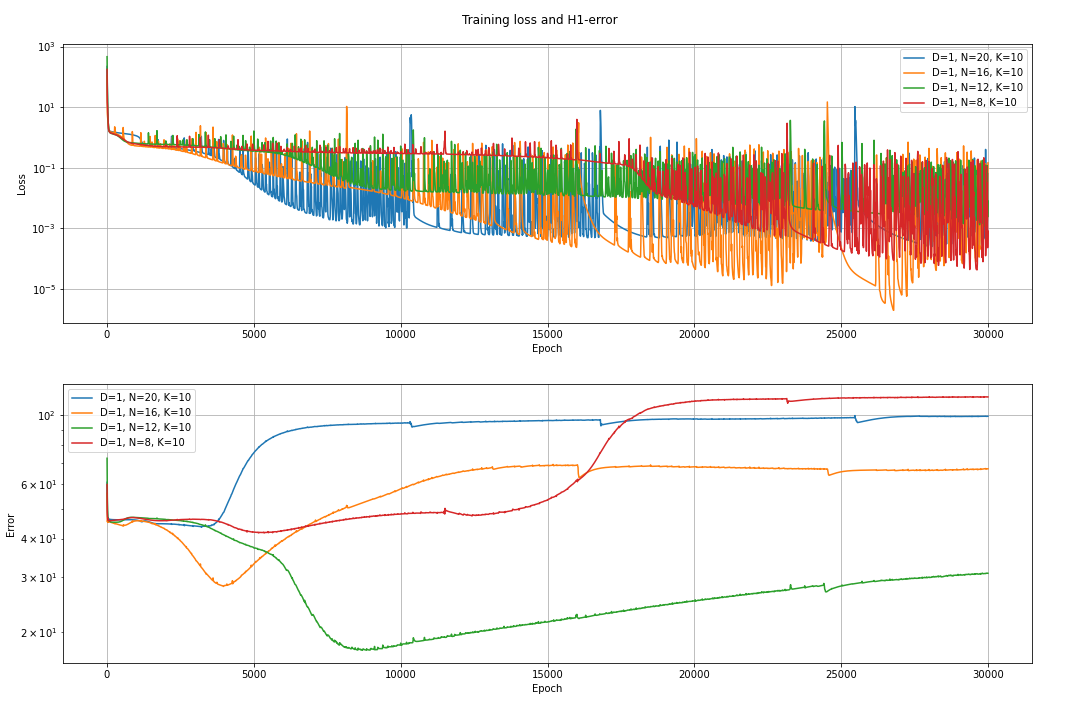
\includegraphics[width=\textwidth]{img/VPINN-Comparison-k8increaseN.png}
        \caption{$k=8$.}
        \label{fig:vpinnsk8increaseN}
    \end{subfigure}
    \caption{Training loss and H1-error with fixed number of test function and increasing width of the network.}
    \label{fig:vpinnsincreaseN}
\end{figure}

To investigate the effect of the width of the network, a similar thing is done with fixing the number of test functions to $K=10$, and training the network for different values of $N$. The results are presented in \autoref{fig:vpinnsincreaseN}. For the lowest wave number $k=2$ in \autoref{fig:vpinnsk2increaseN}, we can see that increasing the width of the network does not bring much to the table. However, the network reaches its minimum H1-error faster. For $k=4$ in \autoref{fig:vpinnsk4increaseN}, we can see that when the width of the network is increased to $16$ or $20$, the unstable behavior emerges even for sufficient number of test functions. For higher wave numbers, the network is not able to converge to the solution with any of these widths, and we can see that increasing the width even makes things worse in \autoref{fig:vpinnsk8increaseN}. These obseervations allow us to conclude that increasing the width of the network cannot heal the need for higher number of test functions, and even requires more test functions in order to converge to the solution.

\begin{figure}[h!]
    \centering
    \begin{subfigure}[b]{0.48\textwidth}
        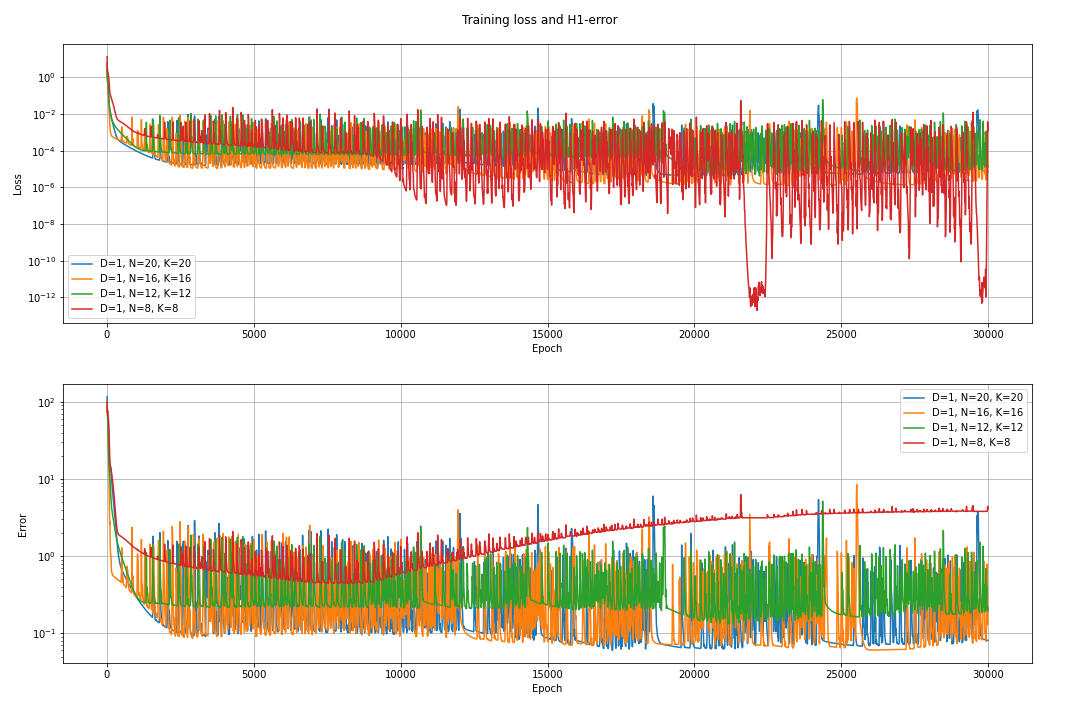
\includegraphics[width=\textwidth]{img/VPINN-Comparison-k2increaseNK.png}
        \caption{$k=2$.}
        \label{fig:vpinnsk2increaseNK}
    \end{subfigure}
    \hfill
    \begin{subfigure}[b]{0.48\textwidth}
        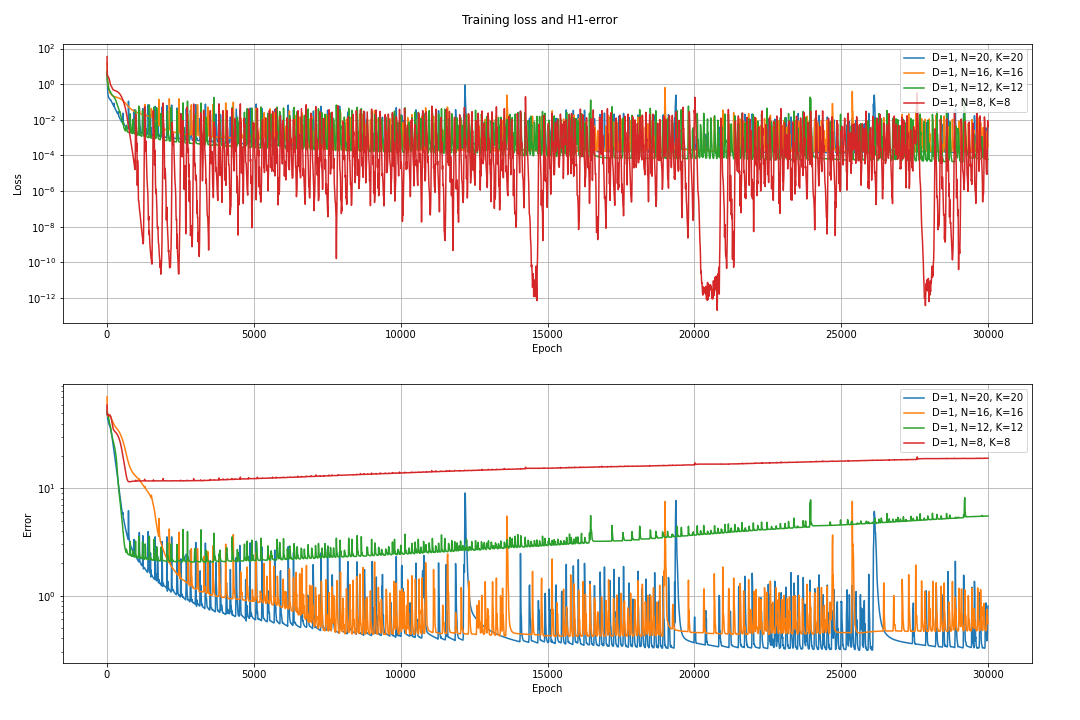
\includegraphics[width=\textwidth]{img/VPINN-Comparison-k4increaseNK.png}
        \caption{$k=4$.}
        \label{fig:vpinnsk4increaseNK}
    \end{subfigure}
    \vfill
    \begin{subfigure}[b]{0.48\textwidth}
        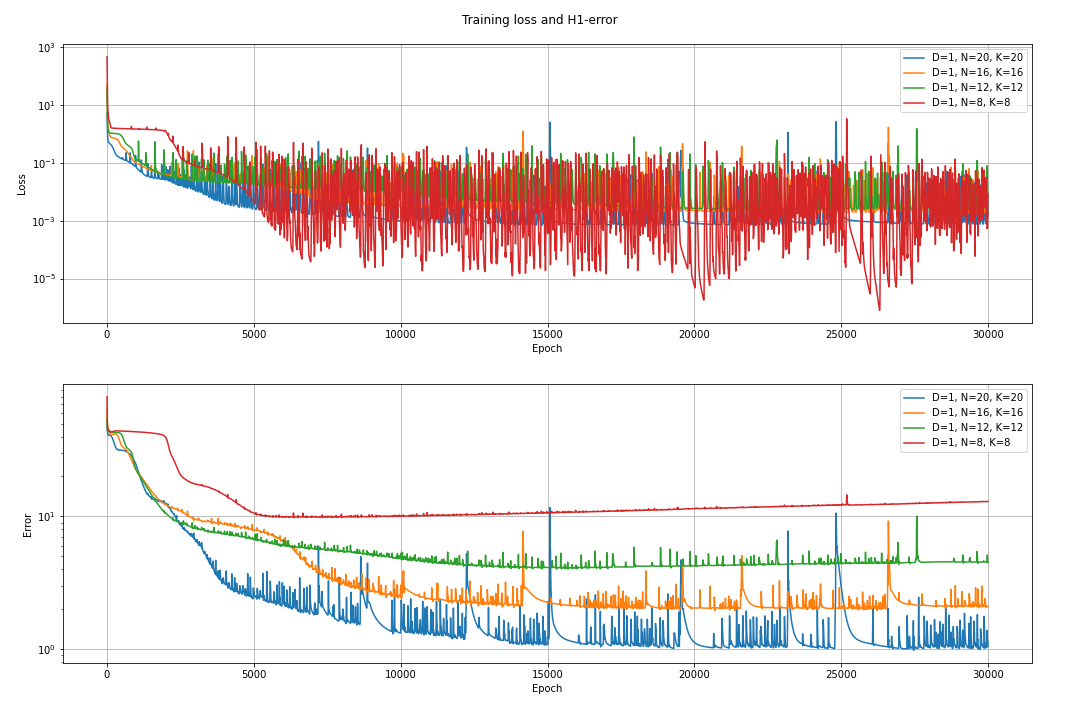
\includegraphics[width=\textwidth]{img/VPINN-Comparison-k6increaseNK.png}
        \caption{$k=6$.}
        \label{fig:vpinnsk6increaseNK}
    \end{subfigure}
    \hfill
    \begin{subfigure}[b]{0.48\textwidth}
        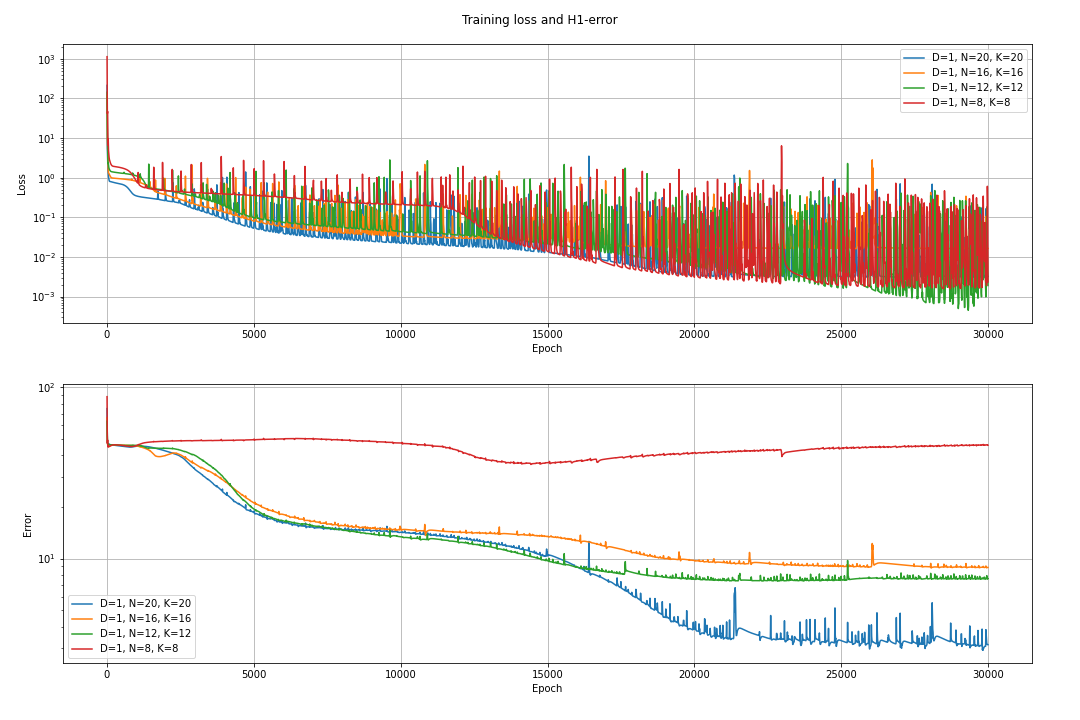
\includegraphics[width=\textwidth]{img/VPINN-Comparison-k8increaseNK.png}
        \caption{$k=8$.}
        \label{fig:vpinnsk8increaseNK}
    \end{subfigure}
    \caption{Training loss and H1-error with fixed number of test function and increasing width of the network.}
    \label{fig:vpinnsincreaseNK}
\end{figure}

In another set of experiments, the width of the network and the number of test functions are kept equal and are increased together. The idea was to treat these two hypermarameters as one parameter since they are bounded together in the FEM scheme. The results are presented in \autoref{fig:vpinnsincreaseNK}. We can see that the final H1-error is consistently improved with increasing both $N$ and $K$ together for all of the wave numbers, but the improvement becomes more evident as the wave number gets higher. These experiments confirm that the best approach is to keep $N$ and $K$ proportional, and increase them together in order to study the convergence rate of this method.

\begin{figure}[h!]
    \centering
    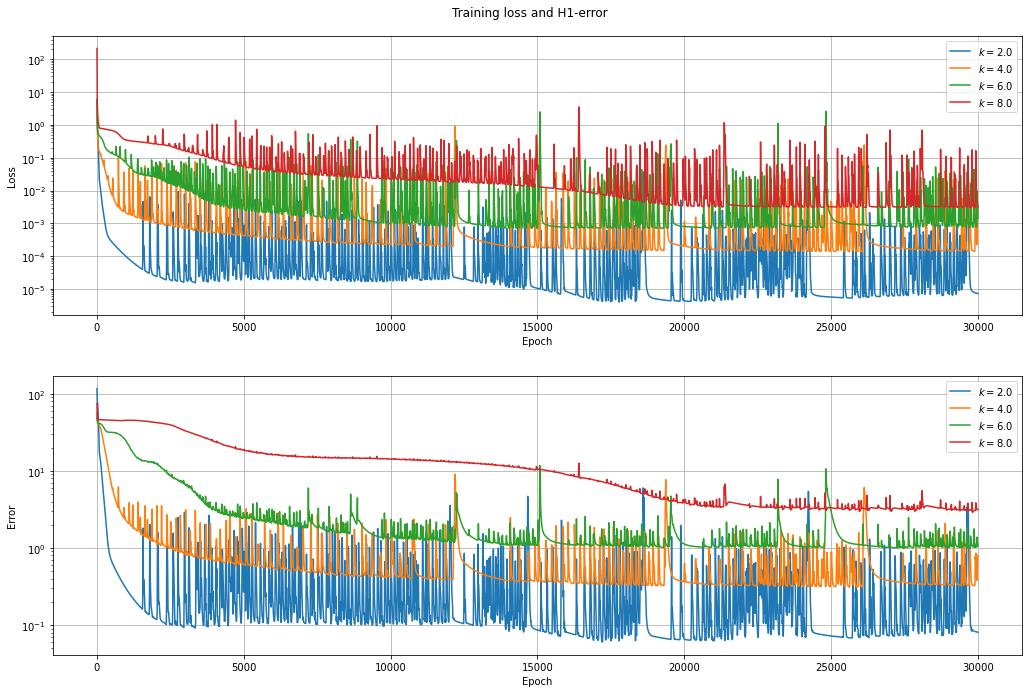
\includegraphics[width=.48\textwidth]{img/VPINN-Comparison-NK20increasek.png}
    \caption{Training loss and H1-error of a shallow network with $N=20$ and $K=20$ for different wave numbers.}
    \label{fig:vpinnsincreasefreq}
\end{figure}

Figure \ref{fig:vpinnsincreasefreq} shows how a quite strong network with $N=K=20$ performs for different wave numbers. Although the network is doing a good job for all of the wave numbers, we can see that as the wave number increases, the accuracy of the final solution decreases, which again implies the need to enrich the network for higher wave numbers.

\subsubsection{Deep Networks}\label{sec:deepnetworks}
From \autoref{eq:vpinnsparameters}, we can see that for deeper neural networks ($D>1$), the number of parameters has a quadratic dependancy on the width of the network, $N$. This gave us the notion that just as increasing $N$ would require more test functions, increasing $D$ might also require the training to be done on more test functions. To address this, we compared the training process for a network with two hidden layers and $N=12$ with different number of test functions. The results are presented in \autoref{fig:vpinnsdeepincreaseK}. We can see that with the same number of test functions as for shallow networks, the model is overfitted to the test functions. While with 20 test functions we can get a better H1-error, further increasing the number of test functions to 28 is not advantageous. We consider 24 test functions adequate for this network structure with 206 parameters. Comparing this number to the number of parameters (50) of the shallow network with the same width, we can assume that the number of adequate test functions scales with the square root of the number of parameters: $K_{adequate} \sim \sqrt{N_p}$.

\begin{figure}[h!]
    \centering
    \begin{subfigure}[b]{0.48\textwidth}
        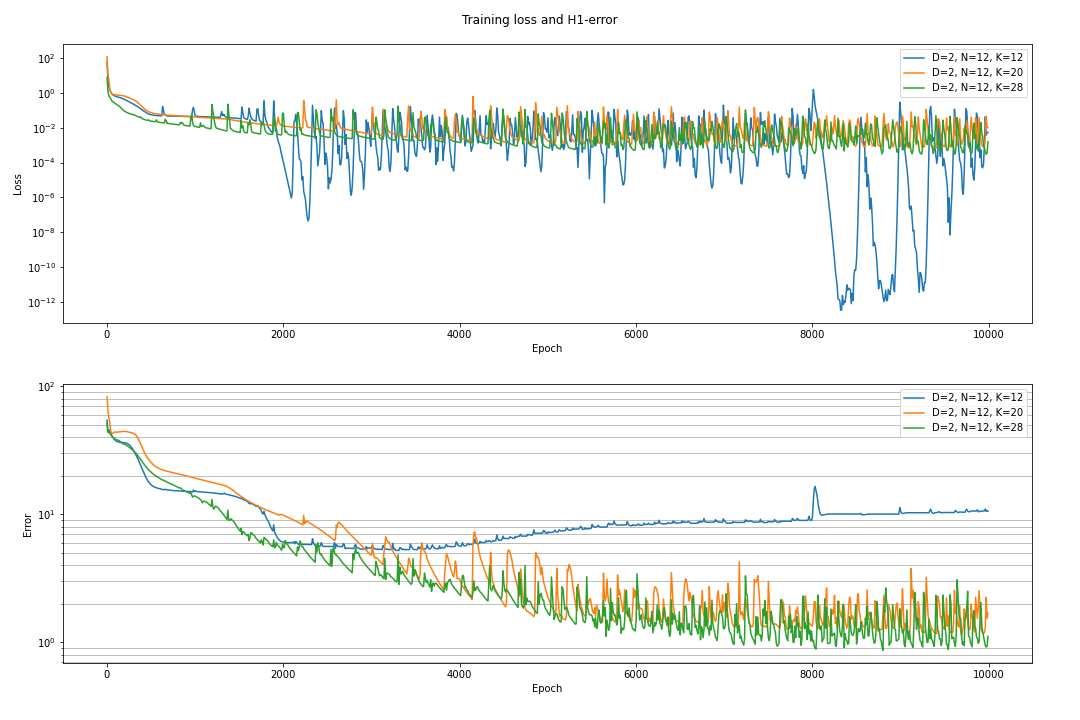
\includegraphics[width=\textwidth]{img/VPINN-Deep-Comparison-k8increaseK.png}
        \caption{Training loss and H1-error of a network with 2 hidden layers and $N=12$ for wave number $k=8.0$, with different number of test functions.}
        \label{fig:vpinnsdeepincreaseK}
    \end{subfigure}
    \hfill
    \begin{subfigure}[b]{0.48\textwidth}
        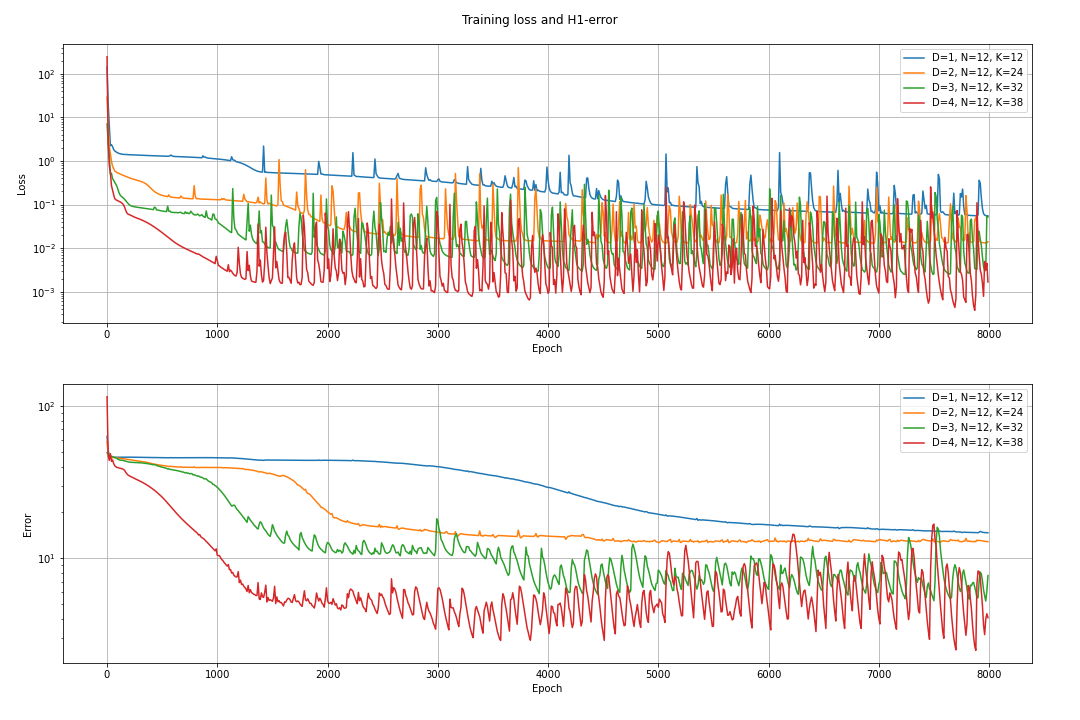
\includegraphics[width=\textwidth]{img/VPINN-Deep-Comparison-k8increaseD.png}
        \caption{Training loss and H1-error of a network with $N=20$ for wave number $k=8.0$, with different depths and number of test functions.}
        \label{fig:vpinnsdeepincreaseD}
    \end{subfigure}
\end{figure}

In \autoref{fig:vpinnsdeepincreaseD}, we keep the width of the network to $N=12$, increase the depth of the netowrk, and increase the number of test functions as $K \simeq 12\sqrt{N_p/50}$ as concluded earlier. It shows that with this approach, both the convergence speed and the final accuracy could be improved very well. Comparing this approach with the best approach in shallow neural networks (increasing the width and the number of test functions equally), we saw that on our CPUs, the deep network with $D=4$, $N=12$ and 38 test functions reaches a decent H1-error in 15 minutes, while a shallow neural network with $20$ nodes and $20$ test functions requires 65 minutes for reaching the same accuracy.

\subsubsection{Least Squares Initialization} \label{sec:lsinitresults}
Instead of random initialization, we initialized the weights and the biases of the shallow network by the method described in \autoref{sec:lsinit} to see how it will affect the training. We trained a shallow network with 20 nodes and 20 test functions for $k=2$, $k=6$, $k=8$, and $k=16$, and compared the training loss and the H1-error to the ones of the same structure with random initialization (as described in previous sections). The learning rate is fixed to $5e{-02}$ in all the trainings, and the same optimizer configurations is used. The results are compared in \autoref{fig:vpinnslsinit}. First of all, we can observe that the initialization is mostly effective for high wave numbers. For $k=2$, although the least-squares initialization gives a good first guess, the random initialization outperforms it both in the final accuracy and in the convergence speed. For other wave numbers, we can see a huge improvement in terms of the convergence speed. For $k=6$, the H1-error hits its minimum in less than 500 epochs, which is reached by random initialized network in around 4000 training epochs. A similar trend could be observed for $k=8$ where the least-squares initialized network reaches $1e{+01}$ H1-error in 500 training epochs, while with random initialization this error is only reached after 15000 epochs. For $k=16$, we can see that the random initialized network fails to converge to the solution but the least-squares initialized performs quite well.

\begin{figure}[h!]
    \centering
    \begin{subfigure}[b]{0.48\textwidth}
        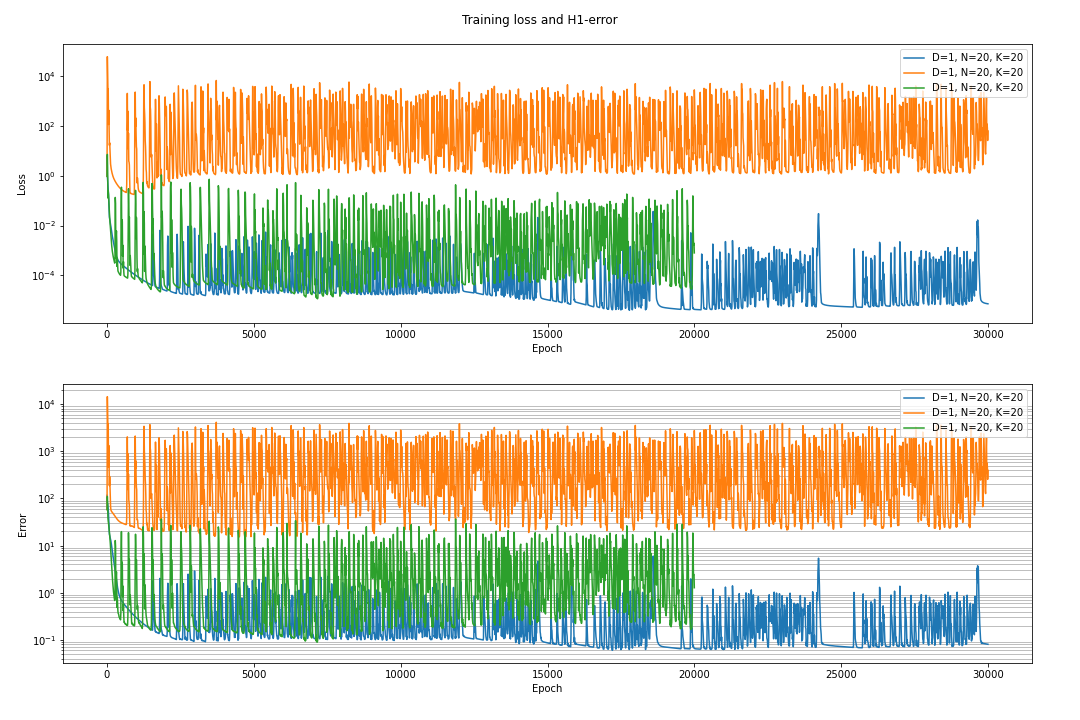
\includegraphics[width=\textwidth]{img/VPINN-Comparison-lsinitk2.png}
        \caption{$k=2$.}
        \label{fig:vpinnslsinitk2}
    \end{subfigure}
    \hfill
    \begin{subfigure}[b]{0.48\textwidth}
        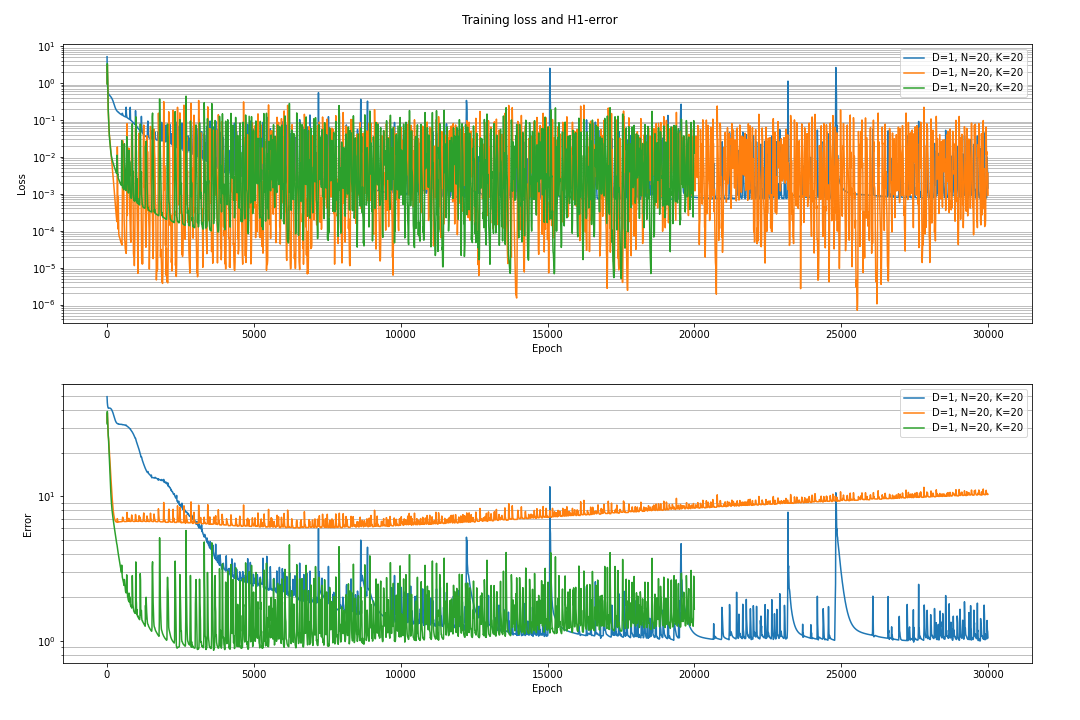
\includegraphics[width=\textwidth]{img/VPINN-Comparison-lsinitk6.png}
        \caption{$k=6$.}
        \label{fig:vpinnslsinitk6}
    \end{subfigure}
    \vfill
    \begin{subfigure}[b]{0.48\textwidth}
        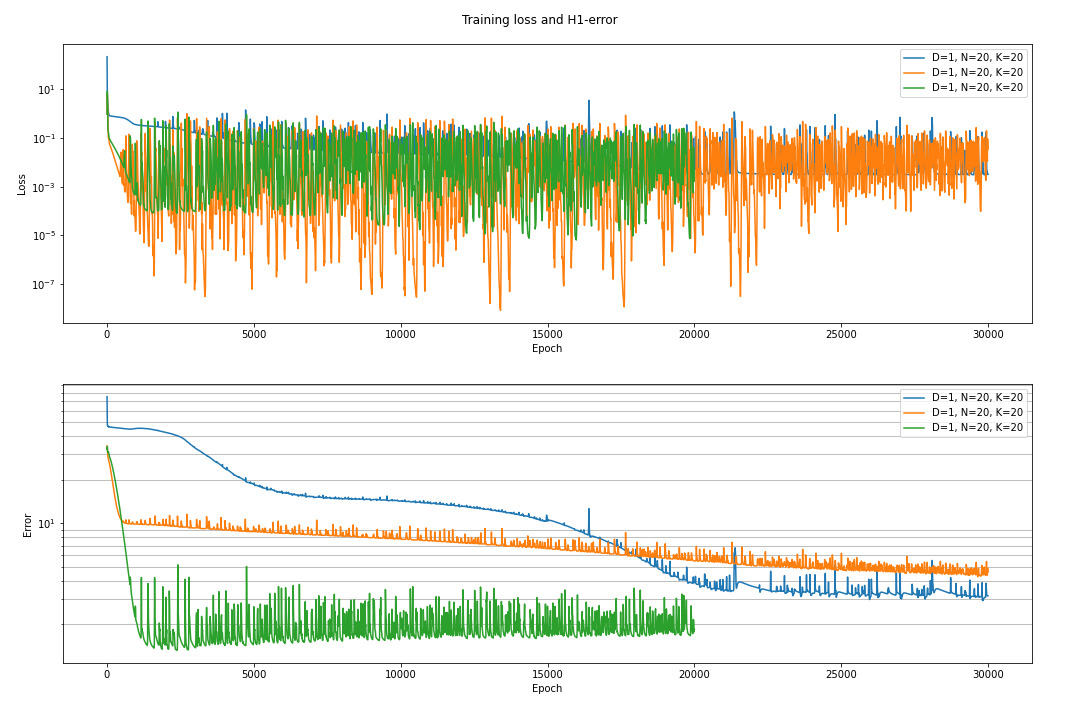
\includegraphics[width=\textwidth]{img/VPINN-Comparison-lsinitk8.png}
        \caption{$k=8$.}
        \label{fig:vpinnslsinitk8}
    \end{subfigure}
    \hfill
    \begin{subfigure}[b]{0.48\textwidth}
        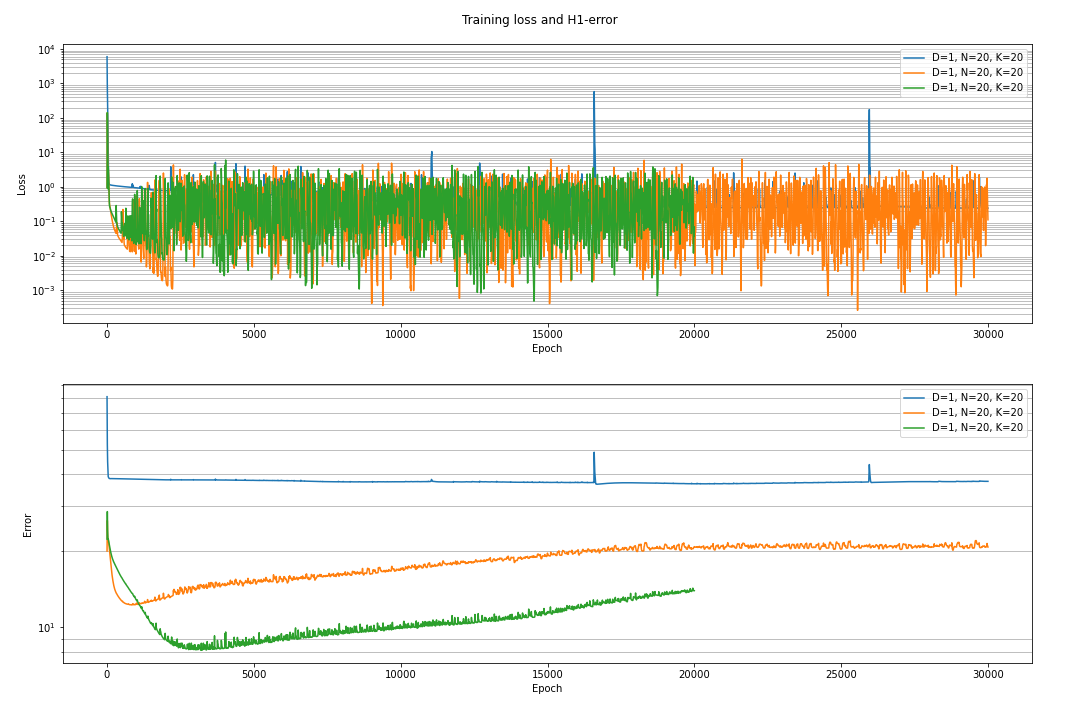
\includegraphics[width=\textwidth]{img/VPINN-Comparison-lsinitk16.png}
        \caption{$k=16$.}
        \label{fig:vpinnslsinitk16}
    \end{subfigure}
    \caption{Training loss and H1-error of the same network structure with random initialization (blue), least-squares initialization (orange), and improved least-squares initialization (green) for different wave numbers.}
    \label{fig:vpinnslsinit}
\end{figure}

However, after a very sharp decrease in the H1-error in the initial epochs, the least-squares initialized networks were not successful in reaching the potential of the network completely, or with a good convergence rate. We can see that for all the wave numbers below $k=16$, the final H1-error is much better with random initialization. This might lie on the fact that although the least-squares initialization gives a solid first guess of the final solution, it might lack the randomness usually demanded by the neural networks to adapt to doing their task perfectly. This could be originated in the initialization of the parameters of the hidden layer, where we set all the weights equally. This issue could be easily solved by adding a noise to these weights. In a slightly different version of this initialization, instead of setting all the weights of the hidden layer to the wave numer $k$, we sampled them from a normal distribution with the mean $k^{0.75}$ and the standard deviation $k^{0.2}$. The green curves in \autoref{fig:vpinnslsinit} correspond to this set of experiments. We can see that this technique improves the training with this initialization impressively. For $k=6.0$, the network with improved initialization hits a minimum H1-error in less than 3000 epochs, compared to 20000 epochs with random initialization. For $k=8$, the minimum error is reached in 2000 epochs, which the randomly initialized network does not reach even in 30000 epochs, and for $k=16$, the best accuracy reached is clearly improved.

Another important aspect regarding the proposed initialization method is that the performance of the first guess is not necessarily improved with increasing the width of the network, $N$. This is simply because of the uniform distribution of $x^{*}$'s, as indicated in \autoref{sec:lsinit}. In fact, for $k=6$, for instance, the least-squares initialized network with 12 nodes resembles the exact solution much better than with 20 nodes. This behavior of the initialization could also be decisive in the instable behavior of the network in Figures \ref{fig:vpinnslsinitk6} and \ref{fig:vpinnslsinitk16}, and explains the better performance for $k=8$ in \autoref{fig:vpinnslsinitk8}. Having a more suitable distribution of the $x^{*}$'s based on the wave number $k$ and the type of source function could solve this issue and improve the initialization method very well.

\subsubsection{Coercive Variational Formulation}\label{sec:coerciveresults}
In order to investigate the behavior of the network using the coercive variational formulation presented in \autoref{sec:coerciveformulation}, we trained a shallow neural network with 20 nodes on the hidden layer and 20 test functions with this formulation, and compared the training process to the original variational formulation. As the coercive formulation requires test functions in $H^2(\Omega)$, the finite element hat functions could not be used for this formulation. Therefore, the first 20 Legendre polynomials, which have global support, are used as test functions. As illustrated in \autoref{fig:coercive}, the coercive formulation with Legendgre polynomials as test functions converges more slowly than the original formulation with hat test functions, but slightly faster than the original formulation with Legendre polynomials. Comparing the time it took for each of these experiments to perform 10000 epochs (on the same device), we can conclude that using global test functions is computationally more expensive than using local test functions, and the coercive formulation is computationally more expensive than the original variational formulation. In the case of $k=8$, the coercive formulation with Legendre test functions took 260 minutes to evolve 10000 epochs, which took only 24 minutes for the original formulation with hat test functions.

\begin{figure}[h!]
    \centering
    \begin{subfigure}[b]{0.48\textwidth}
        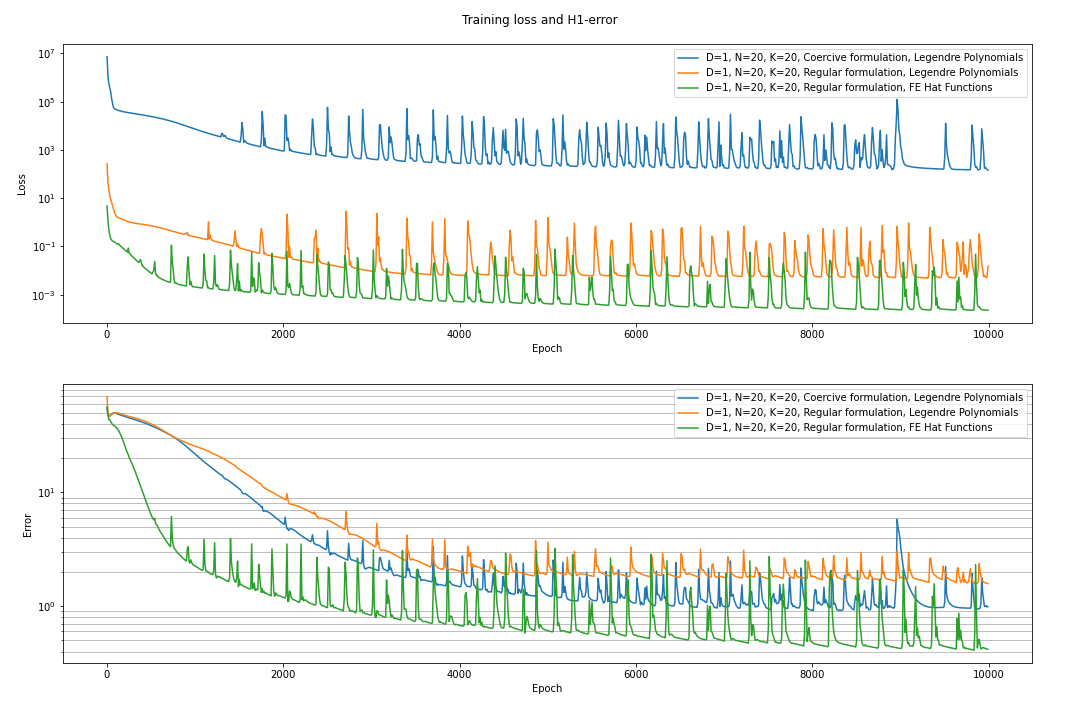
\includegraphics[width=\textwidth]{img/VPINN-Comparison-HFk4.png}
        \caption{$k=4$.}
        \label{fig:coercivek4}
    \end{subfigure}
    \hfill
    \begin{subfigure}[b]{0.48\textwidth}
        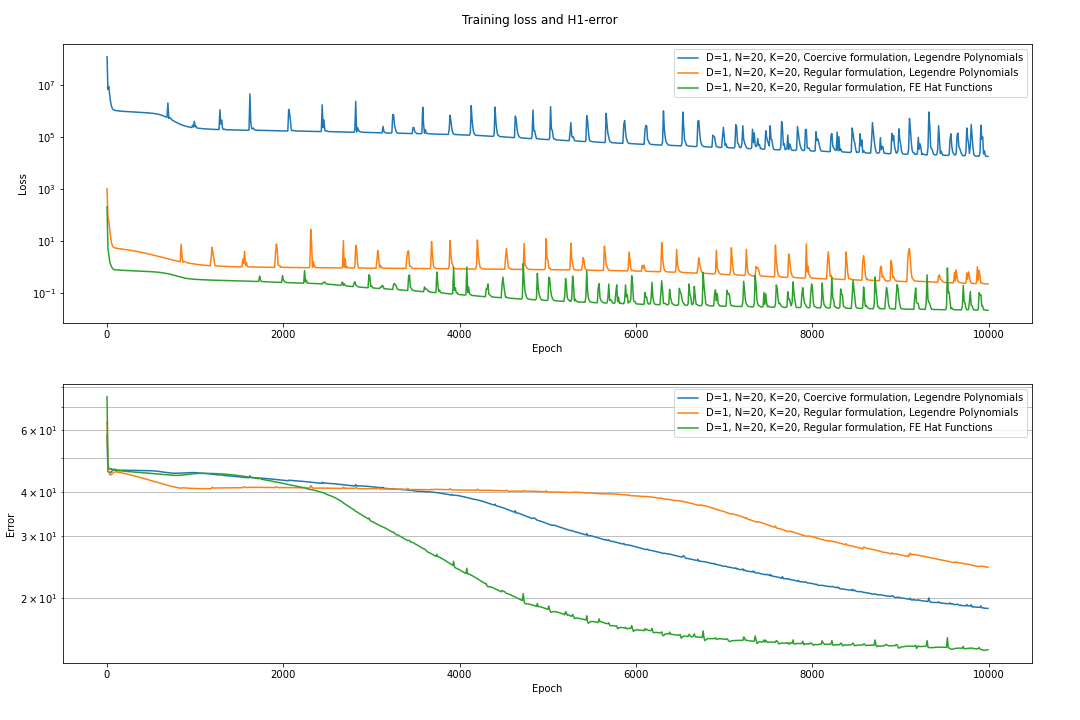
\includegraphics[width=\textwidth]{img/VPINN-Comparison-HFk8.png}
        \caption{$k=8$.}
        \label{fig:coercivek8}
    \end{subfigure}
    \caption{Training loss and H1-error for the same structure with different formulations and test functions.}
    \label{fig:coercive}
\end{figure}

However, the advantages of the coercive formulation reveal themselves when being compared to the regular formulation with Legendre polynomials. Comparing the difference of these two methods for $k=4$ and $k=8$, we can see that as the wave number increases, the advantages of the coercive formulation become more significant. This brings up the idea that using this formulation in conjunction with suitable test functions in $H^2(\Omega)$ with local support could lead to better convergence rates for high wave numbers.

\section{Conclusion}\label{sec:conclusion}
In \autoref{sec:femresults}, we showed that although the finite element scheme could solve the Helmholtz Impedance problem accurately and efficiently, the first-order convergence (in the case of using the hat test functions) only starts after a certain level of refinement, and as the wave number $k$ increases, this critical level of refinement goes higher. This motivated us to implement a VPINNs scheme for this problem and investigate the effect of different configurations of the network on its performance. These observations can eventually be put together to craft some specialized techniques to get a better performance in high wave numbers.

In \autoref{sec:vpinnsshallowresults}, we observed that the hyperbolic tangent is the most suitable activation function for this setup, and kept using this activation function in the rest of the experiments. By doing several experiments with different network widths ($N$) and different number of test functions ($K$), we also observed that the best refinement approach for shallow networks is to increase these two hyper-parameters correlated to each other. In \autoref{sec:deepnetworks}, we investigated the existance of a similar correlation with the depth of the network and concluded that the correlation should be defined on the number of paramters of the network, and proposed to scale the number of test functions with the square root of the number of parameters of the network. We also showed that with adequate width, increasing the depth of the network is a better approach than increasing its width, in terms of convergence time.

In \autoref{sec:lsinitresults}, we investigated the initialization method described in \autoref{sec:lsinit} and showed that a suitable initialization technique could effectively improve the convergence speed of the network. We showed that for $k=8$ with sufficient width and sufficient test functions, the network with suitable initialization could achieve its capacity in 2000 epochs, while with random initialization, even after 30000 epochs it does not reach its capacity. We also pointed out some suggestions for improving this initialization technique such as adapting the biases to the nature of the flow, instead of distributing them uniformly in the domain. In \autoref{sec:coerciveresults}, we compared the convergence rate of the formulation presented in \autoref{sec:coerciveformulation} with the original variational formulation and concluded that the coercive variational formulation could be beneficial in high wave numbers, but it is computationally more expensive in low wave numbers. We also pointed out that using a set of suitable ($H^2(\Omega)$) test functions with local support could speed up the training with this formulation.

In future works, some of the ideas developed in the previous sections could be investigated to see if they help the training or making the network more powerful:
\begin{itemize}
    \item The use of ReLU and similar activation function could be mathematically analyzed and the reasons of their failure should be investigated. Once done, the structure of the network could be changed to take advantage of features of this activation function. As a suggestion, a local version of the ReLU activation function (e.g., ReLU with support in $[0, 1]$) could be applied only on the first hidden layer in order to make the network behave differently in different parts of the domain. This way, depending on where the input of the network is, only some of the nodes in the first layer will be activated. Such a network is implemented in the \texttt{VPINN\_HelmholtzImpedanceRF} class but fails to converge for the same reasons mentioned in \autoref{sec:vpinnsshallowresults}. The results and the detailed implementation are provided in \autoref{app:deeprf}.

    \item Similar to the proposed initialization method in \autoref{sec:lsinit}, the weights of the last layer could be calculated by least-squares on every iteration. Doing this, we will only optimize the parameters of the hidden layers, thus we will solve for the best basis functions that suite the solution. Such methods have been proposed in \cite{cyr2019} and \cite{liu2021}.

    \item Inspired by data augmentation techniques in supervised machine learning, we can interpret the test functions as our data, and try out some similar techniques on the way we use them. It was understood that increasing the number of test functions has the most impact on the computational cost. Therefore, using the test functions more smartly could improve the training in terms of speed and accuracy. Translating the stochastic gradient decent method, we can take the gradient decent steps on a batch of the test functions, instead of summing up the gradients for all of them before taking the step. Doing this, we can also shuffle the order of the test functions on each epoch. Another preposition which could massively increase the capacity of the network without adding significant computational costs, is to randomly choose $K$ test functions among a set of $K'>K$ number of test functions. That is to say, we can, instead of defining $K$ local hat functions and training on all of them, define $K'$ local hat functions, which descretize the domain better, but still keep training on only $K$ of them, randomly chosen on each epoch. Stochastically, the network will be optimized for all the test functions.

    \item Investigating the evolution of the solution throughout the training, we could see that with some configurations, the network manages to capture either the real or the imaginary part of the solution very well, but lacks accuracy in the other part of the solution. The evolution of the solution with random initialzation and with least-squares initialization are available in \autoref{app:evolutions}. Regarding this observation, we suggest that training two networks for each part (imaginary, real) of the solution could be beneficial.

\end{itemize}
